\subsection{ANNIHILATORS. FAITHFUL MODULES. MONOGENOUS MODULES}

DEFINITION 11. The annihilator of a subset S of an A-module E is the set of elements \(\alpha \in \mathbf{A}\) such that \(\alpha x = 0\) for all \(x \in S\) .

The annihilator of S is usually denoted by Ann(S); for a subset S consisting of a single element x, we write Ann(x) instead of Ann(\{x\}) and call Ann(x) the annihilator of x.

The relation \(\alpha x = 0\) may also be expressed by saying that \(x\) is annihilated by \(\alpha\) .

It is immediate that the annihilator of an arbitrary subset S of E is a left ideal of A; for it to be equal to A, it is necessary and sufficient (by virtue of \((\mathbf{M}_{\mathrm{IV}})\) ) that \(S = \{0\}\) . If two subsets S, T of E are such that \(S \subset T\) , the annihilator of T is contained in the annihilator of S. If \((\mathbf{S}_{t})_{t \in I}\) is an arbitrary family of subsets of E, the annihilator of the union \(\bigcup_{t} S_{t}\) is the intersection of the annihilators of the \(S_{t}\) . In particular, the annihilator of a subset S of E is the intersection of the annihilators of the elements of S. To say that an element of E is free is equivalent to saying that its annihilator is \(\{0\}\) . For all \(x \in E\) and all \(\alpha \in A\) , the annihilator of \(\alpha x\) is the set of \(\beta \in A\) such that \(\beta \alpha \in \text{Ann}(x)\) .

The annihilator of a submodule M of E is a two-sided ideal of A; for, if \(\alpha x = 0\) for all \(x \in M\) , then also \(\alpha(\beta x) = 0\) for all \(x \in M\) and all \(\beta \in A\) , hence \(\alpha\beta\) belongs to the annihilator of M for all \(\beta \in A\) . In particular, the annihilator of E is a two-sided ideal of A.

For all \(\alpha \in \mathbf{A}\) , let \(h_{\alpha}\) be the homothety \(x \mapsto \alpha x\) ; it is known that the mapping \(\alpha \mapsto h_{\alpha}\) of \(\mathbf{A}\) into the endomorphism ring \(\mathcal{E} = \operatorname{Hom}_{\mathbf{Z}}(\mathbf{E}, \mathbf{E})\) of the commutative group (without operators) \(\mathbf{E}\) , is a ring homomorphism ( \(\S 2\) , no. 5). The inverse image of 0 under this homomorphism is the annihilator \(\mathfrak{a}\) of \(\mathbf{E}\) ; the image of \(\mathbf{A}\) under the homomorphism \(\alpha \mapsto h_{\alpha}\) is therefore isomorphic to the quotient ring \(\mathbf{A}/\mathfrak{a}\) . The module \(\mathbf{E}\) is called faithful if its annihilator \(\mathfrak{a}\) reduces to 0.

Let E be any A-module, a a two-sided ideal of A contained in Ann(E) and let \(\dot{\alpha}\) be an element of the quotient ring A/a; for all \(x \in E\) , the element \(\alpha x\) is the same for all the \(\alpha \in A\) belonging to the class \(\dot{\alpha} \mod a\) ; if this element is denoted by \(\dot{\alpha}x\) , it is immediately seen that the mapping \((\dot{\alpha}, x) \mapsto \dot{\alpha}x\) defines (with addition on E) an (A/a)-module structure on E. When \(a = \text{Ann}(E)\) , the (A/a)-module E thus defined is faithful; we shall say that it is the faithful module associated with the A-module E. Observe that every submodule of an A-module E is also a submodule of the associated faithful module and conversely.

DEFINITION 12. A module is called monogenous if it is generated by a single element.

Proposition 9 of no. 7 shows that, if E is a monogenous A-module and a is an element generating E, E is identical with the set A.a of \(\xi a\) , where \(\xi\) runs through A.

Examples. (1) Every monogenous group, being commutative (I, § 4, no. 10, Proposition 18), is a monogenous Z-module.

\begin{enumerate}
\def\labelenumi{(\arabic{enumi})}
\setcounter{enumi}{1}
\item
  If A is a commutative ring, the monogenous submodules of the A-module A are just the principal ideals (I, § 8, no. 6) of the ring A.
\item
  Every simple A-module E is monogenous, since the submodule of E generated by an element \(\neq0\) of E is necessarily equal to E.
\end{enumerate}

PROPOSITION 22. Let A be a ring. Every quotient module of \(\mathbf{A}_s\) is monogenous. Conversely, let E be a monogenous A-module, \(c\) a generator of E and a its annihilator; the linear mapping \(\xi \mapsto \xi c\) defines, when passing to the quotient, an isomorphism of \(\mathbf{A}_s / \mathfrak{a}\) onto E.

As \(A_{s}\) is itself monogenous, being generated by 1, the first assertion follows from no. 7, Corollary 1 to Proposition 9. The second is obvious, since \(\xi \mapsto \xi c\) is by hypothesis surjective and has kernel a.

Note that, if A is not commutative, the annihilators of two distinct generators c, \(c'\) of a monogenous A-module E are in general distinct and are also distinct from the annihilator of the module E. On the other hand, if A is commutative, the annihilator of a generator c of E is contained in the annihilator of every element of E and hence is the annihilator of the whole of E.

COROLLARY. Every submodule of a monogenous A-module E is isomorphic to a quotient module b/a where a and b are two left-ideals of A such that \(a \subset b\) . Every quotient module of a monogenous A-module is monogenous.

The second assertion is immediate and the first follows from Proposition 22 and I, § 4, no. 6, Theorem 4.

Note on the other hand that a submodule of a monogenous module is not necessarily monogenous. For example, if A is a commutative ring in which there exist non-principal ideals (VII, §1, no. 1), these ideals are non-monogenous submodules of the monogenous A-module A.

It follows from the definitions that a submodule of an A-module E generated by a family \((a_{t})\) of elements of E is the sum of the monogenous submodules

\(Aa_{t}\) of E; for \((a_{t})\) to be a basis of E, it is necessary and sufficient that each of the \(a_{t}\) be a free element of E and that the sum of the \(Aa_{t}\) be direct.

PROPOSITION 23. Let E be an A-module, the direct sum of an infinite family \((\mathbf{M}_t)_{t\in I}\) of non-zero submodules. For every generating system S of E, \(\operatorname{Card}(\mathbf{S})\geqslant \operatorname{Card}(\mathbf{I})\)

For all \(x \in S\) , let \(C_x\) be the finite set of indices \(i \in I\) such that the component of \(x\) in \(M_i\) is \(\neq 0\) and let \(C = \bigcup_{x \in S} C_x\) . Every \(x \in S\) belongs by definition to the submodule of \(E\) the direct sum of the \(M_i\) for \(i \in C\) and the hypothesis that \(S\) generates \(E\) implies therefore that \(C = I\) ; as \(I\) is by hypothesis infinite, so is \(S\) (Set Theory, III, §5, no. 1, Corollary 1 to Proposition 1); therefore \(\text{Card}(I) = \text{Card}(C) \leqslant \text{Card}(S)\) (Set Theory, III, §6, no. 3, Corollary 3 to Theorem 2).

COROLLARY 1. Under the hypotheses of Proposition 23, suppose that each \(\mathbf{M}_{\iota}\) is monogenous and that \(\mathbf{E}\) is the direct sum of a second family \((\mathrm{N}_{\lambda})_{\lambda \in \mathbf{L}}\) of non-zero monogenous submodules. Then \(\operatorname{Card}(\mathbf{L}) = \operatorname{Card}(\mathbf{I})\) .

If \(b_{\lambda}\) is a generator of \(\mathbf{N}_{\lambda}\) , the set of \(b_{\lambda}\) is a generating system of \(\mathbf{E}\) , hence \(\operatorname{Card}(\mathbf{L}) \geqslant \operatorname{Card}(\mathbf{I})\) . In particular \(\mathbf{L}\) is infinite and, exchanging the roles of \((\mathbf{M}_i)\) and \((\mathbf{N}_{\lambda})\) , similarly \(\operatorname{Card}(\mathbf{I}) \geqslant \operatorname{Card}(\mathbf{L})\) , whence the corollary.

COROLLARY 2. If a module E admits an infinite basis B, every generating system of E has cardinal \(\geqslant\) Card(B) and every basis of E is equipotent to B.

\subsection{CHANGE OF RING OF SCALARS}

Let A, B be two rings and \(\rho\) a homomorphism of the ring B into the ring A. For every A-module E, the external law \((\beta, x) \mapsto \rho(\beta)x\) defines (with addition) a B-module structure said to be associated with \(\rho\) and the A-module structure on E; this B-module is denoted by \(\rho_{*}(\mathbf{E})\) or \(E_{[B]}\) (and even simply E if no confusion can arise). In particular, if B is a subring of A and \(\rho: B \to A\) is the canonical injection, \(E_{[B]}\) is called the B-module obtained by restricting the ring of scalars A to B; by an abuse of language, this expression is also used when the homomorphism \(\rho\) is arbitrary.

If \(\mathbf{F}\) is a submodule of the A-module \(\mathbf{E},\rho_{*}(\mathbf{F})\) is a submodule of \(\rho_{*}(\mathbf{E})\) and \(\rho_{*}(\mathbf{E} / \mathbf{F})\) is equal to \(\rho_{*}(\mathbf{E}) / \rho_{*}(\mathbf{F})\) .

Let E, F be two A-modules; every A-linear mapping \(u: E \rightarrow F\) is also a B-linear mapping \(E_{[B]} \rightarrow F_{[B]}\) denoted by \(\rho_{*}(u)\) ; in other words, there is a canonical injection of Z-modules

\[
\operatorname{Hom} _ {\mathbf {A}} (\mathbf {E}, \mathbf {F}) \rightarrow \operatorname{Hom} _ {\mathbf {B}} (\mathbf {E} _ {[ \mathbf {B} ]}, \mathbf {F} _ {[ \mathbf {B} ]}).\tag{47}
\]

This mapping is not necessarily bijective; in other words a B-linear mapping \(E_{[B]} \rightarrow F_{[B]}\) is not necessarily A-linear. For example, a sub-B-module of \(E_{[B]}\) is not necessarily a sub-A-module of E: if A is a field and B a subfield of A, the vector subspace \(B_{s}\) of the vector B-space \((A_{s})_{[B]}\) is not a vector sub-A-space if \(B \neq A\) .

It is immediate that, for every family \((\mathbf{E}_t)_{t\in I}\) of A-modules, the B-module \(\rho_{*}\left(\prod_{i\in I}\mathbf{E}_{i}\right)\left(\text{resp. } \rho_{*}\left(\bigoplus_{i\in I}\mathbf{E}_{i}\right)\right)\) is equal to \(\prod_{i\in I}\rho_{*}(\mathbf{E}_{i})\) (resp. \(\bigoplus_{i\in I}\rho_{*}(\mathbf{E}_{i})\) ).

Every generating system of \(\rho_{*}(\mathbf{E})\) is a generating system of E but the converse is not necessarily true.

PROPOSITION 24. Let A, B be two rings and \(\rho: \mathbf{B} \to \mathbf{A}\) a ring homomorphism.

\begin{enumerate}
\def\labelenumi{(\roman{enumi})}
\item
  If \(\rho\) is surjective, the canonical mapping (47) is bijective. For every A-module E, every sub-B-module of \(\rho_{*}(\mathbf{E})\) is a sub-A-module of E; every generating system of E is a generating system of \(\rho_{*}(\mathbf{E})\) .
\item
  If \(\rho\) is injective, every free family in the A-module \(\mathbf{E}\) is a free family in the B-module \(\rho_{*}(\mathbf{E})\) .
\end{enumerate}

The proposition follows immediately from the definitions.

Note that even if \(\rho\) is injective, a free family in \(\rho_{*}(\mathbf{E})\) is not necessarily free in \(\mathbf{E}\) .

*For example, 1 and \(\sqrt{2}\) do not form a free system in \(\mathbf{R}\) considered as a vector \(\mathbf{R}\) -space, although they form a free system in \(\mathbf{R}\) considered as a vector \(\mathbf{Q}\) -space (cf.~Remark 1).*

PROPOSITION 25. Let A, B be two rings, \(\rho: \mathbf{B} \to \mathbf{A}\) a ring homomorphism and E an A-module. Let \((\alpha_{\lambda})_{\lambda \in L}\) be a generating system (resp. free family of elements, basis) of A considered as a left B-module. Let \((a_{\mu})_{\mu \in M}\) be a generating system (resp. free family of elements, basis) of the A-module E. Then \((\alpha_{\lambda}a_{\mu})_{(\lambda,\mu) \in L \times M}\) is a generating system (resp. (when \(\rho\) is injective) free family of elements, basis) of the B-module \(\rho_{*}(\mathbf{E})\) .

If \(x = \sum_{\mu \in \mathbf{M}} \gamma_{\mu} a_{\mu}\) , where \(\gamma_{\mu} \in \mathbf{A}\) and \((\alpha_{\lambda})\) is a generating system of \(\mathbf{A}\) , we may write \(\gamma_{\mu} = \sum_{\lambda \in L} \rho(\beta_{\lambda \mu}) \alpha_{\lambda}\) , with \(\beta_{\lambda \mu} \in \mathbf{B}\) , for all \(\mu \in \mathbf{M}\) , whence \(x = \sum_{\lambda, \mu} \rho(\beta_{\lambda \mu}) \alpha_{\lambda} a_{\mu}\) . On the other hand, if \((\alpha_{\lambda})\) and \((a_{\mu})\) are free families, a relation \(\sum_{\lambda, \mu} \rho(\beta_{\lambda \mu}) \alpha_{\lambda} a_{\mu} = 0\) , with \(\beta_{\lambda \mu} \in \mathbf{B}\) , may be written \(\sum_{\mu \in M} \left( \sum_{\lambda \in L} \rho(\beta_{\lambda \mu}) \alpha_{\lambda} \right) a_{\mu} = 0\) ; it thus implies \(\sum_{\lambda \in L} \rho(\beta_{\lambda \mu}) \alpha_{\lambda} = 0\) for all \(\mu \in M\) and therefore \(\beta_{\lambda \mu} = 0\) for all \(\lambda, \mu\) if \(\rho\) is injective.

COROLLARY. If A is a finitely generated left B-module and E a finitely generated left A-module, \(\rho_{*}(\mathbf{E})\) is a finitely generated left A-module.

Let C be a third ring, \(\rho':\mathbf{C}\to\mathbf{B}\) a ring homomorphism and \(\rho''=\rho\circ\rho'\) the composite homomorphism. It follows immediately from the definitions that \(\rho_{*}^{\prime \prime}(\mathbf{E}) = \rho_{*}^{\prime}(\rho_{*}(\mathbf{E}))\) for every A-module E. In particular, if \(\rho\) is an isomorphism of B onto A, then \(\mathbf{E} = \rho_{*}^{\prime}(\rho_{*}(\mathbf{E}))\) , where \(\rho^{\prime}\) denotes the inverse isomorphism of \(\rho\) .

Remarks. (1) Let K be a field and A a subring of K with the following property: for every finite family \((\xi_{i})_{1\leqslant i\leqslant n}\) of elements of K, there exists a \(\gamma\in A\) which is non-zero and such that \(\gamma\xi_{i}\in A\) for \(1\leqslant i\leqslant n\) (a hypothesis which is always satisfied when A is commutative and K is the field of fractions of A). Let E be a vector space over K and \(E_{[A]}\) the A-module obtained by restricting the ring of scalars to A. Then, if a family \((x_{\lambda})_{\lambda\in L}\) is free in \(E_{[A]}\) it is also free in E. Attention may be confined to the case where \(L=\{1,n\}\) ; if there were a relation \(\sum_{i=1}^{n} \xi_i x_i = 0\) with \(\xi_i \in \mathbf{K}\) , the \(\xi_i\) not all zero, it would follow that for all \(\beta \in \mathbf{A}, \sum_{i=1}^{n} (\beta \xi_i) x_i = 0\) . By hypothesis we can suppose \(\beta \neq 0\) in \(\mathbf{A}\) such that \(\beta \xi_{i} = \alpha_{i}\) belongs to A for all \(i\) ; but the relation \(\sum_{i=1}^{n} \alpha_{i} x_{i} = 0\) is contrary to the hypothesis, the \(\alpha_{i}\) being not all zero.

\begin{enumerate}
\def\labelenumi{(\arabic{enumi})}
\setcounter{enumi}{1}
\tightlist
\item
  If the ring homomorphism \(\rho: \mathbf{B} \to \mathbf{A}\) is surjective and \(\mathfrak{b}\) is its kernel (so that \(\mathbf{A}\) is canonically identified with \(\mathbf{B} / \mathfrak{b}\) ), then, for every A-module \(\mathbf{E}\) , \(\mathfrak{b}\) is contained in the annihilator of \(\rho_*(\mathbf{E})\) and \(\mathbf{E}\) is the A-module derived from \(\rho_*(\mathbf{E})\) by the process defined in no. 12.
\end{enumerate}

Let A, B be two rings and \(\rho: \mathbf{B} \to \mathbf{A}\) a homomorphism. Let E be an A-module and F a B-module; a B-linear mapping \(u: \mathbf{F} \to \rho_{*}(\mathbf{E})\) (also called a B-linear mapping of F into E if no confusion arises) is also called a semi-linear mapping (relative to \(\rho\) ) of the B-module F into the A-module E; it is also said that the ordered pair \((u, \rho)\) is a dimorphism of F into E; this therefore means that, for \(x \in \mathbf{F}\) , \(y \in \mathbf{F}\) and \(\beta \in \mathbf{B}\) ,

\[
\left\{ \begin{array}{l} u (x + y) = u (x) + u (y) \\ u (\beta x) = \rho (\beta) u (x). \end{array} \right.\tag{48}
\]

The set \(\operatorname{Hom}_{\mathbf{B}}(\mathbf{F},\rho_{*}(\mathbf{E}))\) of B-linear mappings of \(\mathbf{F}\) into \(\mathbf{E}\) is also written as \(\operatorname{Hom}_{\mathbf{B}}(\mathbf{F},\mathbf{E})\) if no confusion can arise.

When \(\rho\) is an isomorphism of B onto A, the relation \(u(\beta x) = \rho(\beta) u(x)\) for all \(\beta \in B\) may also be written as \(u(\rho'(\alpha)x) = \alpha x\) for all \(\alpha \in A\) , where \(\rho'\) denotes the inverse isomorphism of \(\rho\) ; to say that \(u\) is semi-linear for \(\rho\) is then equivalent to saying that \(u\) is an A-linear mapping of \(\rho_*(F)\) into E.

Example. It has been seen (no. 1) that a homothety \(h_{\alpha} \colon x \mapsto \alpha x\) on an A-module \(\mathbf{E}\) is not necessarily a linear mapping. But if \(\alpha\) is invertible, \(h_{\alpha}\) is a semi-linear mapping (which is moreover bijective) relative to the inner automorphism \(\xi \mapsto \alpha \xi \alpha^{-1}\) of \(\mathbf{A}\) , for \(\alpha(\lambda x) = (\alpha \lambda \alpha^{-1})(\alpha x)\) .

Let C be a third ring, \(\rho':\mathrm{C}\to\mathrm{B}\) a homomorphism and G a C-module. If \(v:\mathrm{G}\to\mathrm{F}\) is a semi-linear mapping relative to \(\rho'\) , the composition \(w=u\circ v\) is a semi-linear mapping of G into E relative to the homomorphism \(\rho''=\rho\circ\rho'\) . If \(\rho\) is an isomorphism and \(u:\mathrm{F}\to\mathrm{E}\) is a bijective semi-linear mapping relative to \(\rho\) , the inverse mapping \(u':\mathrm{E}\to\mathrm{F}\) is a semi-linear mapping relative to the inverse isomorphism \(\rho':\mathrm{A}\to\mathrm{B}\) of \(\rho\) .

It is thus seen that, for the species of structure defined by giving on an ordered pair (A, E) of sets a ring structure on A and a left A-module structure on E, the dimorphisms \((u, \phi)\) can be taken as morphisms (Set Theory, IV, §2, no. 1); we shall always assume in what follows that this choice of morphisms has been made.

Remark (3). Let \(A_{1}\) , \(A_{2}\) be two rings, \(A = A_{1} \times A_{2}\) their product and let \(e_{1} = (1, 0)\) , \(e_{2} = (0, 1)\) in A, so that \(A_{1}\) and \(A_{2}\) are canonically identified with the two-sided ideals \(Ae_{1}\) and \(Ae_{2}\) of A. For every A-module E, \(e_{1}E\) and \(e_{2}E\) are sub-A-modules \(E_{1}\) , \(E_{2}\) of E, annihilated respectively by \(e_{2}\) and \(e_{1}\) , so that, canonically identifying \(A/Ae_{2}\) with \(A_{1}\) and \(A/Ae_{1}\) with \(A_{2}\) , \(E_{1}\) (resp. \(E_{2}\) ) is given an \(A_{1}\) -module (resp. \(A_{2}\) -module) structure. Moreover, E is the direct sum of \(E_{1}\) and \(E_{2}\) , for every \(x \in E\) can be written as \(x = e_{1}x + e_{2}x\) and the relation \(e_{1}x = e_{2}y\) implies \(e_{1}x = e_{1}^{2}x = e_{1}e_{2}y = 0\) . Conversely, for every ordered pair consisting of an \(A_{1}\) -module \(F_{1}\) and an \(A_{2}\) -module \(F_{2}\) , let \(E_{1}\) be the A-module \((p_{1}) * (F_{1})\) , \(E_{2}\) the A-module \((p_{2}) * (F_{2})\) , \(p_{1}\) and \(p_{2}\) being the projections of A onto \(A_{1}\) and \(A_{2}\) respectively; then in the A-module \(E = E_{1} \oplus E_{2}\) , \(E_{1} = e_{1}E\) , \(E_{2} = e_{2}E\) . The study of A-modules is thus reduced to that of \(A_{1}\) -modules and that of \(A_{2}\) -modules. In particular, every submodule M of E is of the form \(M_{1} \oplus M_{2}\) , where \(M_{1} = e_{1}M\) and \(M_{2} = e_{2}M\) .

\subsection{MULTIMODULES}

Let A, B be two rings and consider on a set E two left module structures with the same additive law and whose ring of operators are respectively A and B; let \(\mathcal{E}\) be the endomorphism ring of the additive group E and for all \(\alpha \in A\) (resp. \(\beta \in B\) ) let \(h_{\alpha}\) (resp. \(h_{\beta}^{\prime}\) ) denote the element \(x \mapsto \alpha x\) (resp. \(x \mapsto \beta x\) ) of \(\mathcal{E}\) . Clearly the three following properties are equivalent: (a) \(h_{\alpha} \circ h_{\beta}^{\prime} = h_{\beta}^{\prime} \circ h_{\alpha}\) for all \(\alpha\) and \(\beta\) ; (b) the image of A under the homomorphism \(a \mapsto h_{\alpha}\) is contained in \(\operatorname{Hom}_{\mathbf{B}}(\mathbf{E}, \mathbf{E})\) ; (c) the image of B under the homomorphism \(\beta \mapsto h_{\beta}^{\prime}\) is contained in \(\operatorname{Hom}_{\mathbf{A}}(\mathbf{E}, \mathbf{E})\) . When the A-module (resp. B-module) structure in question is a right module structure, the ring A (resp. B) must be replaced in (b) (resp. (c)) by \(\mathbf{A}^{0}\) (resp. \(\mathbf{B}^{0}\) ). The above properties can be expressed by saying that the two (left or right) module structures defined on E are compatible.

DEFINITION 13. Let \((\mathbf{A}_{\lambda})_{\lambda \in \mathbf{L}}, (\mathbf{B}_{\mu})_{\mu \in \mathbf{M}}\) be two families of rings; an \(((\mathbf{A}_{\lambda}), (\mathbf{B}_{\mu}))\) -multimodule (or multimodule over the families of rings \((\mathbf{A}_{\lambda})_{\lambda \in \mathbf{L}}, (\mathbf{B}_{\mu})_{\mu \in \mathbf{M}})\) is a set E with, for each \(\lambda \in \mathbf{L}\) , a left \(\mathbf{A}_{\lambda}\) -module structure and, for each \(\mu \in \mathbf{M}\) , a right \(\mathbf{B}_{\mu}\) -module structure, all these module structures being compatible with one another.

When the family \((\mathbf{B}_{\mu})\) (resp. \((\mathbf{A}_{\lambda})\) ) is empty, E is called a left (resp. right) multimodule. When \(\operatorname{Card}(\mathbf{L}) + \operatorname{Card}(\mathbf{M}) = 2\) , we say ``bimodule'' instead of ``multimodule''; it is then often convenient to consider (as can always be done by replacing a ring of operators by its opposite, cf.~no. 1) a bimodule as having a left module structure with respect to a ring A and a right module structure with respect to a ring B, the permutability of the laws then being expressed by the relation

\begin{enumerate}
\def\labelenumi{(\arabic{enumi})}
\setcounter{enumi}{48}
\tightlist
\item
\end{enumerate}

\[
\alpha (x \beta) = (\alpha x) \beta \quad \text { for } x \in \mathbf {E}, \alpha \in \mathbf {A}, \beta \in \mathbf {B}.
\]

It is then also said that \(\mathbf{E}\) is an (A, B)-bimodule.

Two multimodule structures on a set E are said to be compatible if all the module structures on E which define one or the other of these multimodule structures are compatible with one another.

Examples. (1) On a ring A the module structures of \(A_{s}\) and \(A_{d}\) are compatible and A can therefore be considered canonically as an (A, A)-bimodule.

\begin{enumerate}
\def\labelenumi{(\arabic{enumi})}
\setcounter{enumi}{1}
\tightlist
\item
  A left A-module E has a canonical left module structure over the ring \(\operatorname{End}_{\mathbf{A}}(\mathbf{E})\) and the A-module and \(\operatorname{End}_{\mathbf{A}}(\mathbf{E})\) -module structures on E are compatible.
\end{enumerate}

Clearly when E is a multimodule over two families \((\mathbf{A}_{\lambda})_{\lambda\in L},(\mathbf{B}_{\mu})_{\mu\in M}\) of rings, E is also a multimodule over any two subfamilies \((\mathbf{A}_{\lambda})_{\lambda\in L},(\mathbf{B}_{\mu})_{\mu\in M'}\) , where the \(A_{\lambda}\) -module and \(B_{\mu}\) -module structures for \(\lambda\in L'\) and \(\mu\in M'\) are those initially given.

Since multimodules are particular examples of commutative groups with operators, the results of nos. 2 to 10 (cf.~no. 10, Remark) can be applied to them; in particular, if E, F are two \(((A_{\lambda}), (B_{\mu}))\) -multimodules, a homomorphism \(u: E \to F\) is a mapping which is an \(A_{\lambda}\) -homomorphism for all \(\lambda \in L\) and a \(B_{\mu}\) -homomorphism for all \(\mu \in M\) . The stable subgroups of an \(((A_{\lambda}), (B_{\mu}))\) -multimodule are \(((A_{\lambda}), (B_{\mu}))\) -multimodules (called submultimodules), as also are the quotients by such subgroups (called quotient multimodules); similarly for products and direct sums.

Let E be an \(((A_{\lambda}), (B_{\mu}))\) -multimodule and for each \(\lambda \in L\) (resp. \(\mu \in M\) ) let \(\phi_{\lambda}: A_{\lambda}' \to A_{\lambda}\) (resp. \(\psi_{\mu}: B_{\mu}' \to B_{\mu}\) ) be a ring homomorphism; clearly the \(A_{\lambda}'\) -module structures associated with the \(\phi_{\lambda}\) and the \(A_{\lambda}\) -module structures given on E and the \(B_{\mu}'\) -module structures associated with the \(\psi_{\mu}\) and the \(B_{\lambda}\) -module structures given on E are compatible with one another and hence define on E an \(((A_{\lambda}')\) , \((B_{\mu}')\) )-multimodule structure, said to be associated with the given \(((A_{\lambda})\) , \((B_{\mu})\) )-multimodule structure and the \(\phi_{\lambda}\) and \(\psi_{\mu}\) .

If E, F are two \(((A_{\lambda}), (B_{\mu}))\) -multimodules, the additive group of homomorphisms of E into F is denoted by \(\operatorname{Hom}_{(A_{\lambda}), (B_{\mu})}(E, F)\) (or simply \(\operatorname{Hom}(E, F)\) ). Formulae (6) to (8) of no. 2 are obviously valid for \(((A_{\lambda}), (B_{\mu}))\) -multimodule homomorphisms and, in particular, \(\operatorname{Hom}(E, E) = \operatorname{End}(E)\) has a ring structure;

moreover \(\operatorname{Hom}(\mathbf{E},\mathbf{F})\) has a canonical left \(\operatorname{End}(\mathbf{F})\) -module structure and right \(\operatorname{End}(\mathbf{E})\) -module structure, these two structures being compatible; in other words, \(\operatorname{Hom}(\mathbf{E},\mathbf{F})\) has a canonical (End(F), End(E))-bimodule structure.

Suppose now that E has a multimodule structure whose rings of left (resp. right) operators are on the one hand the \(A_{\lambda}\) for \(\lambda \in L\) (resp. the \(B_{\mu}\) for \(\mu \in M\) ) and on the other the rings of another family \((\mathbf{A}_{\lambda'}')_{\lambda' \in L'}\) (resp. \((\mathbf{B}_{\mu'}')_{\mu' \in M'}\) ). Suppose similarly that F has a multimodule structure whose rings of left (resp. right) operators are on the one hand the \(A_{\lambda}\) for \(\lambda \in L\) (resp. the \(B_{\mu}\) for \(\mu \in M\) ) and on the other the rings of another family \((\mathbf{A}_{\lambda''})_{\lambda'' \in L''}\) (resp. \((\mathbf{B}_{\mu''})_{\mu'' \in M''}\) ); to abbreviate we shall say that E is an \(((\mathbf{A}_{\lambda}), (\mathbf{A}_{\lambda'}'); (\mathbf{B}_{\mu}), (\mathbf{B}_{\mu'})\) -multimodule and F an \(((\mathbf{A}_{\lambda}), (\mathbf{A}_{\lambda''}); (\mathbf{B}_{\mu}), (\mathbf{B}_{\mu''}))\) -multimodule. Consider E and F as \(((\mathbf{A}_{\lambda}), (\mathbf{B}_{\mu}))\) -multimodules, thus restricting the operators to the subfamilies \((\mathbf{A}_{\lambda})\) and \((\mathbf{B}_{\mu})\) . By what was said at the beginnings of this no., the multimodule structures given on E and F define canonically ring homomorphisms

\[
\mathrm{A} _ {\lambda^ {\prime}} ^ {\prime} \rightarrow \operatorname{End} _ {(\mathrm{A} _ {\lambda}), (\mathrm{B} _ {\mu})} (\mathrm{E}), \quad \mathrm{B} _ {\mu^ {\prime}} ^ {\prime 0} \rightarrow \operatorname{End} _ {(\mathrm{A} _ {\lambda}), (\mathrm{B} _ {\mu})} (\mathrm{E}),
\]

\[
\mathrm{A} _ {\lambda^ {\prime \prime}} ^ {\prime \prime} \rightarrow \operatorname{End} _ {(\mathrm{A} _ {\lambda}), (\mathrm{B} _ {\mu})} (\mathrm{F}), \quad \mathrm{B} _ {\mu^ {\prime \prime}} ^ {\prime \prime} \rightarrow \operatorname{End} _ {(\mathrm{A} _ {\lambda}), (\mathrm{B} _ {\mu})} (\mathrm{F});
\]

moreover, two elements of \(\operatorname{End}_{(\mathbf{A}_{\lambda}), (\mathbf{B}_{\mu})}(\mathbf{E})\) (resp. \(\operatorname{End}_{(\mathbf{A}_{\lambda}), (\mathbf{B}_{\mu})}(\mathbf{F})\) ) respective images of elements of two distinct rings among the \(\mathbf{A}_{\lambda'}'\) or the \(\mathbf{B}_{\mu'}^{0}\) (resp. the \(\mathbf{A}_{\lambda''}\) or the \(\mathbf{B}_{\mu''}^{0}\) ) are permutable; it follows that the above homomorphisms define on \(\operatorname{Hom}_{(\mathbf{A}_{\lambda}), (\mathbf{B}_{\mu})}(\mathbf{E}, \mathbf{F})\) a multimodule structure whose rings of left operators are the \(\mathbf{A}_{\lambda''}\) ( \(\lambda'' \in \mathbf{L}''\) ) and the \(\mathbf{B}_{\mu'}'\) ( \(\mu' \in \mathbf{M}'\) ) and whose rings of right operators are the \(\mathbf{A}_{\lambda'}'\) ( \(\lambda' \in \mathbf{L}'\) ) and the \(\mathbf{B}_{\mu''}^{0}(\mu'' \in \mathbf{M}'')\) .

If now \(\mathbf{E}'\) is an \(((\mathbf{A}_{\lambda}), (\mathbf{A}_{\lambda'}^{\prime}) ; (\mathbf{B}_{\mu}), (\mathbf{B}_{\mu'}^{\prime}))\) -multimodule and \(\mathbf{F}'\) an \(((\mathbf{A}_{\lambda}), (\mathbf{A}_{\lambda''}^{\prime}) ; (\mathbf{B}_{\mu}), (\mathbf{B}_{\mu''}^{\prime}))\) -multimodule, \(\mathrm{Hom}_{(\mathbf{A}_{\lambda}), (\mathbf{B}_{\mu})}(\mathbf{E}', \mathbf{F}')\) is an

\[
\left(\left(\mathrm{A} _ {\lambda^ {\prime \prime}} ^ {\prime \prime}\right), \left(\mathrm{B} _ {\mu^ {\prime}} ^ {\prime}\right): \left(\mathrm{A} _ {\lambda^ {\prime}} ^ {\prime}\right), \left(\mathrm{B} _ {\mu^ {\prime \prime}} ^ {\prime \prime}\right)\right) - \text { multimodule };
\]

if \(u: \mathbf{E}' \to \mathbf{E}\) , \(v: \mathbf{F} \to \mathbf{F}'\) are multimodule homomorphisms,

\[
\operatorname{Hom} (u, v): \operatorname{Hom} _ {\left(\mathrm{A} _ {\lambda}\right), \left(\mathrm{B} _ {\mu}\right)} (\mathrm{E}, \mathrm{F}) \rightarrow \operatorname{Hom} _ {\left(\mathrm{A} _ {\lambda}\right), \left(\mathrm{B} _ {\mu}\right)} \left(\mathrm{E} ^ {\prime}, \mathrm{F} ^ {\prime}\right)
\]

is defined as in no. 2 and is a multimodule homomorphism.

Remarks. (1) Let F be an A-module and C the centre of the ring A; as central homotheties commute with all homotheties, F has a bimodule structure whose rings of left operators are A and C. If E is another A-module, \(\operatorname{Hom}_{\mathbf{A}}(\mathbf{E}, \mathbf{F})\) has therefore a canonical C-module structure (where, for \(f \in \operatorname{Hom}_{\mathbf{A}}(\mathbf{E}, \mathbf{F})\) and \(\gamma \in C\) , \(\gamma f\) is the homomorphism \(x \mapsto \gamma f(x)\) ); if \(E'\) , \(F'\) are two A-modules, \(u: E' \to E\) , \(v: F \to F'\) two A-homomorphisms, the mapping \(\operatorname{Hom}(u, v)\) is C-linear.

\begin{enumerate}
\def\labelenumi{(\arabic{enumi})}
\setcounter{enumi}{1}
\tightlist
\item
  Let E be a left A-module; as A has a canonical (A, A)-bimodule structure, so has the direct sum \(\mathbf{A}^{(\mathrm{T})}\) for any indexing set T; by the above, \(\mathrm{Hom}_{\mathbf{A}}(\mathbf{A}_{s}^{\mathrm{(T)}},\mathbf{E})\) has a canonical left A-module structure arising from the right A-module structure on \(\mathbf{A}_{s}^{\mathrm{(T)}}\) : for \(f\in\mathrm{Hom}_{\mathbf{A}}(\mathbf{A}_{s}^{\mathrm{(T)}},\mathbf{E})\) and \(\alpha\in\mathbf{A},\alpha f\) is the linear mapping \(x\mapsto f(x\alpha)\) . Corollary 2 to Proposition 17 of no. 11 defines a canonical mapping \(j_{\mathbf{E},\mathbf{T}}\) from the product module \(\mathbf{E}^{\mathrm{T}}\) to \(\mathrm{Hom}_{\mathbf{A}}(\mathbf{A}_{s}^{\mathrm{(T)}},\mathbf{E})\) , the image under \(j_{\mathbf{E},\mathbf{T}}\) of a family \((x_{t})_{t\in\mathbf{T}}\) being the linear mapping \(f:\mathbf{A}_{s}^{\mathrm{(T)}}\to\mathbf{E}\) such that \(f(e_{t})=x_{t}\) for all \(t\in\mathbf{T}\) (where \((e_{t})\) is the canonical basis of \(\mathbf{A}_{s}^{\mathrm{(T)}}\) ); it is known (loc. cit.) that \(j_{\mathbf{E},\mathbf{T}}\) is bijective and it follows from the definition given above of the A-module structure on \(\mathrm{Hom}_{\mathbf{A}}(\mathbf{A}_{s}^{\mathrm{(T)}},\mathbf{E})\) that \(j_{\mathbf{E},\mathbf{T}}\) is A-linear. Finally, if \(u:\mathbf{E}\to\mathbf{F}\) is an A-module homomorphism, the diagram
\end{enumerate}

\[
\begin{array}{c} \mathrm {E^ {T}} \xrightarrow {j _ {\mathrm{E,T}}} \operatorname{Hom} _ {\mathrm{A}} (\mathrm{A} _ {s} ^ {(\mathrm{T})}, \mathrm{E}) \\ u ^ {\mathrm{T}} \Biggl \downarrow \qquad \qquad \qquad \qquad \qquad \qquad \qquad \qquad \qquad \qquad \qquad \qquad \qquad \qquad \qquad \qquad \qquad \qquad \qquad \qquad \qquad \qquad \qquad \qquad \qquad \qquad \qquad \text {Hom(1,u)} \\ \mathrm {F^ {T}} \xrightarrow {j _ {\mathrm{F,T}}} \operatorname{Hom} _ {\mathrm{A}} (\mathrm{A} _ {s} ^ {(\mathrm{T})}, \mathrm{F}) \end{array}\tag{50}
\]

is commutative.

Note that when T consists of a single element, \(j_{E}:E \to \operatorname{Hom}_{A}(A_{s}, E)\) is just the mapping \(x \mapsto \theta_{x}\) defined in no. 2, Example 1.

\section{MODULES OF LINEAR MAPPINGS. DUALITY}

\subsection{\texorpdfstring{PROPERTIES OF \(\operatorname{Hom}_{\mathbf{A}}(\mathbf{E}, \mathbf{F})\) RELATIVE TO EXACT SEQUENCES}{PROPERTIES OF \textbackslash operatorname\{Hom\}\_\{\textbackslash mathbf\{A\}\}(\textbackslash mathbf\{E\}, \textbackslash mathbf\{F\}) RELATIVE TO EXACT SEQUENCES}}

THEOREM 1. Let A be a ring, E', E, E'' three A-modules and u: E' → E, v: E → E'' two homomorphisms. For the sequence

\[
\mathrm{E} ^ {\prime} \stackrel {u} {\longrightarrow} \mathrm{E} \stackrel {v} {\longrightarrow} \mathrm{E} ^ {\prime \prime} \longrightarrow 0\tag{1}
\]

to be exact, it is necessary and sufficient that, for every A-module F, the sequence

\[
0 \longrightarrow \operatorname{Hom} (\mathrm{E} ^ {\prime \prime}, \mathrm{F}) \stackrel {v} {\longrightarrow} \operatorname{Hom} (\mathrm{E}, \mathrm{F}) \stackrel {\bar {u}} {\longrightarrow} \operatorname{Hom} (\mathrm{E} ^ {\prime}, \mathrm{F})\tag{2}
\]

(where \(\bar{u} = \mathrm{Hom}(u, 1_{\mathbf{F}})\) , \(\bar{v} = \mathrm{Hom}(v, 1_{\mathbf{F}})\) ) be exact.

Suppose that sequence (1) is exact. If \(w \in \operatorname{Hom}(\mathbf{E}^{\prime \prime}, \mathbf{F})\) and \(\bar{v}(w) = w \circ v = 0\) , then \(w = 0\) since \(v\) is surjective. Sequence (2) is therefore exact at \(\operatorname{Hom}(\mathbf{E}^{\prime \prime}, \mathbf{F})\) . We show that it is exact at \(\operatorname{Hom}(\mathbf{E}, \mathbf{F})\) . \(\bar{u} \circ \bar{v} = \operatorname{Hom}(v \circ u, 1_{\mathbf{F}})\) (§ 1, no. 2, formula (10)) and \(v \circ u = 0\) since sequence (1) is exact at E. Therefore \(\bar{u} \circ \bar{v} = 0\) , that is \(\operatorname{Im}(\bar{v}) \subset \operatorname{Ker}(\bar{u})\) . On the other hand, if \(w \in \operatorname{Ker}(\bar{u})\) , then \(w \circ u = 0\) and hence \(\operatorname{Ker}(w) \supset \operatorname{Im}(u)\) . But as sequence (1) is exact at E, \(\operatorname{Im}(u) = \operatorname{Ker}(v)\) and hence \(\operatorname{Ker}(w) \supset \operatorname{Ker}(v)\) ; as \(v\) is surjective, it follows from § 1, no. 3, Remark that there exists a \(w' \in \operatorname{Hom}(\mathbf{E}^{\prime \prime}, \mathbf{F})\) such that

\begin{enumerate}
\def\labelenumi{(\arabic{enumi})}
\setcounter{enumi}{3}
\tightlist
\item
\end{enumerate}

\(w = w' \circ v = \bar{v}(w')\) . Therefore \(\operatorname{Ker}(\bar{u}) \subset \operatorname{Im}(\bar{v})\) , which completes the proof that sequence (2) is exact.

Conversely, suppose that (2) is exact for every A-module F. As \(\bar{u} \circ \bar{v} = \operatorname{Hom}(v \circ u, 1_{\mathbf{F}}) = 0\) , \(w \circ v \circ u = 0\) for every homomorphism \(w: \mathrm{E}'' \to \mathrm{F}\) . Taking \(\mathrm{F} = \mathrm{E}''\) and \(w = 1_{\mathbf{E}''}\) , it is seen first that \(v \circ u = 0\) and hence \(u(\mathrm{E}') \subset \operatorname{Ker}(v)\) . Now take \(\mathrm{F} = \operatorname{Coker}(u)\) and let \(\phi: \mathrm{E} \to \mathrm{F} = \mathrm{E}/u(\mathrm{E}')\) be the canonical mapping. Then \(\bar{u}(\phi) = \phi \circ u = 0\) by definition and hence there exists a \(\psi \in \operatorname{Hom}(\mathrm{E}''\) , F) such that \(\phi = \bar{v}(\psi) = \psi \circ v\) ; this obviously implies \(u(\mathrm{E}') = \operatorname{Ker}(\phi) \supset \operatorname{Ker}(v)\) , which proves that sequence (1) is exact at E. Finally, let \(\theta\) be the canonical homomorphism of \(\mathrm{E}''\) onto \(\mathrm{F} = \mathrm{E}''/v(\mathrm{E})\) ; then \(\bar{v}(\theta) = \theta \circ v = 0\) , hence \(\theta = 0\) ; therefore, \(\mathrm{F} = \{0\}\) and \(v\) is surjective. Sequence (1) is therefore exact at \(\mathrm{E}''\) .

COROLLARY. For an A-linear mapping \(u: \mathbf{E} \to \mathbf{F}\) to be surjective (resp. bijective, resp. zero), it is necessary and sufficient that, for every A-module \(\mathbf{G}\) , the mapping \(\operatorname{Hom}(u, 1_{\mathbf{G}}): \operatorname{Hom}(\mathbf{F}, \mathbf{G}) \to \operatorname{Hom}(\mathbf{E}, \mathbf{G})\) be injective (resp. bijective, resp. zero).

It suffices to apply Theorem 1 to the case where \(\mathbf{E}'' = \{0\}\) (resp. \(\mathbf{E}' = \{0\}\) resp. \(\mathbf{E}'' = \mathbf{E}\) and \(v = 1_{\mathbb{E}}\) ).

Note that starting from an exact sequence

\[
0 \longrightarrow \mathrm{E} ^ {\prime} \stackrel {u} {\longrightarrow} \mathrm{E} \stackrel {v} {\longrightarrow} \mathrm{E} ^ {\prime \prime} \longrightarrow 0
\]

the corresponding sequence

\[
0 \longrightarrow \operatorname{Hom} (\mathrm{E} ^ {\prime \prime}, \mathrm{F}) \stackrel {\bar {v}} {\longrightarrow} \operatorname{Hom} (\mathrm{E}, \mathrm{F}) \stackrel {\bar {u}} {\longrightarrow} \operatorname{Hom} (\mathrm{E} ^ {\prime}, \mathrm{F}) \longrightarrow 0
\]

is not necessarily exact, in other words, the homomorphism \(\bar{u}\) is not necessarily surjective. If \(E'\) is identified with a submodule of E, this means that a linear mapping of \(E'\) into F cannot always be extended to a linear mapping of E into F (Exercises 11 and 12). However:

PROPOSITION 1. If the exact sequence of linear mappings

\[
0 \longrightarrow \mathrm{E} ^ {\prime} \stackrel {u} {\longrightarrow} \mathrm{E} \stackrel {v} {\longrightarrow} \mathrm{E} ^ {\prime \prime} \longrightarrow 0\tag{3}
\]

splits (in other words, if \(u(\mathbf{E}')\) is a direct factor of \(\mathbf{E}\) ) the sequence

\[
0 \longrightarrow \operatorname{Hom} (\mathrm{E} ^ {\prime \prime}, \mathrm{F}) \stackrel {\bar {v}} {\longrightarrow} \operatorname{Hom} (\mathrm{E}, \mathrm{F}) \stackrel {\bar {u}} {\longrightarrow} \operatorname{Hom} (\mathrm{E} ^ {\prime}, \mathrm{F}) \longrightarrow 0
\]

is exact and splits. Conversely, if, for every \(A\) -module \(F\) , sequence (4) is exact, sequence (3) splits.

If the exact sequence (3) splits, there exists a linear retraction \(u': \mathbf{E} \to \mathbf{E}'\) associated with \(u\) (§ 1, no. 9, Proposition 15); if

\[
\bar {u} ^ {\prime} = \operatorname{Hom} (u ^ {\prime}, 1 _ {\mathrm{F}}): \operatorname{Hom} (\mathrm{E} ^ {\prime}, \mathrm{F}) \rightarrow \operatorname{Hom} (\mathrm{E}, \mathrm{F}),
\]

the fact that \(u' \circ u\) is the identity implies that \(\bar{u} \circ \bar{u}'\) is the identity (§ 1, no. 2, formula (10)) and hence the first assertion follows from § 1, no. 9, Proposition 15. Conversely, suppose sequence (4) is exact for \(F = E'\) . Then there exists an element \(f \in \operatorname{Hom}(E, E')\) such that \(f \circ u = 1_{E'}\) , and the conclusion follows from § 1, no. 9, Proposition 15.

Note that the first assertion of Proposition 1 can also be considered as a special case of §1, no. 6, Corollary 1 to Proposition 6, canonically identifying \(\operatorname{Hom}(\mathbf{E}',\mathbf{F}) \oplus \operatorname{Hom}(\mathbf{E}''\) , \(\mathbf{F}\) ) with \(\operatorname{Hom}(\mathbf{E}' \oplus \mathbf{E}''\) , \(\mathbf{F}\) ) by means of the Z-linear mapping \(\operatorname{Hom}(p',\mathbf{l}_{\mathbf{F}}) + \operatorname{Hom}(p'',\mathbf{l}_{\mathbf{F}})\) , where \(p':\mathbf{E}' \oplus \mathbf{E}'' \to \mathbf{E}'\) and \(p'':\mathbf{E}' \oplus \mathbf{E}'' \to \mathbf{E}''\) are the canonical projections.

THEOREM 2. Let A be a ring, F', F, F'' three A-modules and u: F' → F, v: F → F'' two homomorphisms. For the sequence

\[
0 \longrightarrow \mathrm{F} ^ {\prime} \stackrel {v} {\longrightarrow} \mathrm{F} \stackrel {u} {\longrightarrow} \mathrm{F} ^ {\prime \prime}\tag{5}
\]

to be exact, it is necessary and sufficient that, for every A-module E, the sequence

\[
0 \longrightarrow \operatorname{Hom} (\mathrm{E}, \mathrm{F} ^ {\prime}) \stackrel {\bar {u}} {\longrightarrow} \operatorname{Hom} (\mathrm{E}, \mathrm{F}) \stackrel {\bar {v}} {\longrightarrow} \operatorname{Hom} (\mathrm{E}, \mathrm{F} ^ {\prime \prime})\tag{6}
\]

(where \(\bar{u} = \operatorname{Hom}(1_{\mathbf{E}}, u)\) , \(\bar{v} = \operatorname{Hom}(1_{\mathbf{E}}, v)\) ) be exact.

Suppose that the sequence (5) is exact. Note first that

\[
\bar {v} \circ \bar {u} = \operatorname{Hom} (1 _ {\mathrm{E}}, v \circ u) = 0
\]

(II, § 1, no. 2, formula (10)) since \(v \circ u = 0\) . The image of Hom(E, F') under \(\bar{u}\) is therefore contained in the kernel N of \(\bar{v}\) ; let \(f\) be the homomorphism of the Z-module Hom(E, F') into N whose graph is equal to that of \(\bar{u}\) ; it is necessary to prove that \(f\) is bijective and hence to define a mapping \(g: \mathrm{N} \to \mathrm{Hom}(\mathrm{E}, \mathrm{F}')\) such that \(f \circ g\) and \(g \circ f\) are the identity mappings. For this, let \(w\) be an element of N, that is a linear mapping \(w: \mathrm{E} \to \mathrm{F}\) such that \(v \circ w = 0\) . The latter relation is equivalent to \(w(\mathrm{E}) \subset \mathrm{Ker}(v) = u(\mathrm{F}')\) by hypothesis, hence, since \(u\) is injective, there exists one and only one linear mapping \(w': \mathrm{E} \to \mathrm{F}'\) such that \(w = u \circ w'\) and we take \(g(w) = w'\) ; it is immediately verified that \(g\) satisfies the desired conditions.

Conversely, suppose that sequence (6) is exact for every A-module E. As \(\operatorname{Hom}(1_{\mathbf{E}}, v \circ u) = \bar{v} \circ \bar{u} = 0\) , then \(v \circ u \circ w = 0\) for every homomorphism \(w: E \to F'\) . Taking \(E = F'\) and \(w = 1_{F'}\) , it is seen first that \(v \circ u = 0\) and hence \(u(F') \subset \operatorname{Ker}(v)\) . Now we take \(E = \operatorname{Ker}(v)\) and let \(\phi: E \to F\) be the canonical injection. Then \(\bar{v}(\phi) = v \circ \phi = 0\) by definition and hence there exists \(\psi \in \operatorname{Hom}(E, F')\) such that \(\phi = \bar{u}(\psi) = u \circ \psi\) , which obviously implies \(\operatorname{Ker}(v) \subset u(F')\) and completes the proof of the exactness of (5) at F. Finally, if \(\theta\) is the identity mapping of \(\operatorname{Ker} u\) , then \(\bar{u}(\theta) = 0\) , hence \(\theta = 0\) and \(\operatorname{Ker} u = \{0\}\) , which proves the exactness of (5) at \(F'\) .

Remark. (1) Theorem 2 allows us, for every submodule \(\mathbf{F}'\) of \(\mathbf{F}\) , to identify \(\operatorname{Hom}(\mathbf{E}, \mathbf{F}')\) with a sub- \(\mathbf{Z}\) -module of \(\operatorname{Hom}(\mathbf{E}, \mathbf{F})\) . When this identification is made, then, for every family \((\mathbf{M}_{\lambda})\) of submodules of \(\mathbf{F}\)

\[
\operatorname{Hom} \left(\mathrm{E}, \bigcap_ {\lambda} \mathrm{M} _ {\lambda}\right) = \bigcap_ {\lambda} \operatorname{Hom} (\mathrm{E}, \mathrm{M} _ {\lambda})
\]

for if \(u \in \operatorname{Hom}(\mathbf{E}, \mathbf{F})\) belongs to each of the \(\operatorname{Hom}(\mathbf{E}, \mathbf{M}_{\lambda})\) , then, for all \(x \in \mathbf{E}\) , \(u(x) \in \mathbf{M}_{\lambda}\) for all \(\lambda\) and hence \(u\) maps \(\mathbf{E}\) into \(\bigcap_{\lambda} \mathbf{M}_{\lambda}\) .

COROLLARY. For an A-linear mapping \(u: \mathbf{E} \to \mathbf{F}\) to be injective, it is necessary and sufficient that, for every A-module \(\mathbf{G}\) , the mapping \(\operatorname{Hom}(1_{\mathbf{G}}, u): \operatorname{Hom}(\mathbf{G}, \mathbf{E}) \to \operatorname{Hom}(\mathbf{G}, \mathbf{F})\) be injective.

It suffices to apply Theorem 2 to the case where \(\mathbf{F}' = \{0\}\) .

Starting from an exact sequence

\[
0 \longrightarrow \mathrm{F} ^ {\prime} \stackrel {u} {\longrightarrow} \mathrm{F} \stackrel {v} {\longrightarrow} \mathrm{F} ^ {\prime \prime} \longrightarrow 0
\]

the corresponding sequence

\[
0 \longrightarrow \operatorname{Hom} (\mathrm{E}, \mathrm{F} ^ {\prime}) \stackrel {\bar {u}} {\longrightarrow} \operatorname{Hom} (\mathrm{E}, \mathrm{F}) \stackrel {\bar {v}} {\longrightarrow} \operatorname{Hom} (\mathrm{E}, \mathrm{F} ^ {\prime \prime}) \longrightarrow 0
\]

is not necessarily exact, in other words \(\bar{v}\) is not necessarily surjective. If \(F'\) is identified with a submodule of F and \(F''\) with the quotient module \(F/F'\) , this means that a linear mapping of E into \(F''\) is not necessarily of the form \(v \circ w\) , where w is a linear mapping of E into F. However:

PROPOSITION 2. If the exact sequence

\[
0 \longrightarrow \mathrm{F} ^ {\prime} \stackrel {u} {\longrightarrow} \mathrm{F} \stackrel {v} {\longrightarrow} \mathrm{F} ^ {\prime \prime} \longrightarrow 0\tag{7}
\]

splits (in other words, if \(u(\mathbf{F}')\) is a direct factor of \(\mathbf{F}\) ), the sequence

\[
0 \longrightarrow \operatorname{Hom} (\mathrm{E}, \mathrm{F} ^ {\prime}) \stackrel {\bar {u}} {\longrightarrow} \operatorname{Hom} (\mathrm{E}, \mathrm{F}) \stackrel {\bar {v}} {\longrightarrow} \operatorname{Hom} (\mathrm{E}, \mathrm{F} ^ {\prime \prime}) \longrightarrow 0\tag{8}
\]

is exact and splits. Conversely, if sequence (8) is exact for every A-module E, the exact sequence (7) splits.

The first assertion follows from the fact that

\[
\operatorname{Hom} (\mathbf {E}, \mathbf {F} ^ {\prime}) \oplus \operatorname{Hom} (\mathbf {E}, \mathbf {F} ^ {\prime \prime})
\]

is canonically identified with \(\operatorname{Hom}(\mathbf{E}, \mathbf{F}' \oplus \mathbf{F}'')\) by means of the \(\mathbf{Z}\) -linear mapping \(\operatorname{Hom}(1_{\mathbb{E}}, j') + \operatorname{Hom}(1_{\mathbb{E}}, j'')\) , \(j': \mathbf{F}' \to \mathbf{F}' \oplus \mathbf{F}''\) and \(j'': \mathbf{F}'' \to \mathbf{F}' \oplus \mathbf{F}''\) being the canonical injections (§ 1, no. 6, Corollary 1 to Proposition 6). Conversely, if sequence (8) is exact for \(\mathbf{E} = \mathbf{F}''\) , there is an element \(g \in \operatorname{Hom}(\mathbf{F}''\) , \(\mathbf{F}\) ) such that \(v \circ g = 1_{\mathbf{F}''}\) and the conclusion follows from § 1, no. 9, Proposition 15.

Remark (2). The results of this no. are valid without modification for all commutative groups with operators.

\subsection{PROJECTIVE MODULES}

DEFINITION 1. An A-module P is called projective if, for every exact sequence \(\mathbf{F}' \to \mathbf{F} \to \mathbf{F}''\) of A-linear mapping, the sequence

\[
\operatorname{Hom} (\mathrm{P}, \mathrm{F} ^ {\prime}) \rightarrow \operatorname{Hom} (\mathrm{P}, \mathrm{F}) \rightarrow \operatorname{Hom} (\mathrm{P}, \mathrm{F} ^ {\prime \prime})
\]

is exact.

PROPOSITION 3. For an A-module P, the direct sum of a family of submodules \((\mathbf{M}_{t})\) , to be projective, it is necessary and sufficient that each of the \(\mathbf{M}_{t}\) be projective.

For every A-module homomorphism \(u: \mathbf{E} \to \mathbf{F}\) ,

\[
\operatorname{Hom} \left(1 _ {\mathrm{P}}, u\right): \operatorname{Hom} (\mathrm{P}, \mathrm{E}) \rightarrow \operatorname{Hom} (\mathrm{P}, \mathrm{F})
\]

is identified with \(\prod_{i}\operatorname{Hom}(1_{M_i},u)\) (§ 1, no. 6, Corollary 1 to Proposition 6); the conclusion thus follows from Definition 1 and § 1, no. 5, Proposition 5 (ii).

COROLLARY. Every free A-module is projective.

It suffices by Proposition 3 to show that \(A_{s}\) is projective, which follows immediately from the commutativity of diagram (50) of §1, no. 14.

PROPOSITION 4. Let P be an A-module. The following properties are equivalent:

\begin{enumerate}
\def\labelenumi{(\alph{enumi})}
\item
  P is projective.
\item
  For every exact sequence \(0 \to \mathbf{F}' \to \mathbf{F} \to \mathbf{F}'' \to 0\) of A-linear mappings, the sequence
\end{enumerate}

\[
0 \rightarrow \operatorname{Hom} (\mathrm{P}, \mathrm{F} ^ {\prime}) \rightarrow \operatorname{Hom} (\mathrm{P}, \mathrm{F}) \rightarrow \operatorname{Hom} (\mathrm{P}, \mathrm{F} ^ {\prime \prime}) \rightarrow 0
\]

is exact.

\begin{enumerate}
\def\labelenumi{(\alph{enumi})}
\setcounter{enumi}{2}
\item
  For every surjective A-module homomorphism \(u: \mathbf{E} \to \mathbf{E}''\) and every homomorphism \(f: \mathbf{P} \to \mathbf{E}''\) , there exists a homomorphism \(g: \mathbf{P} \to \mathbf{E}\) such that \(f = u \circ g\) (it is said that \(f\) can be ``lifted'' to a homomorphism of \(\mathbf{P}\) into \(\mathbf{E}\) ).
\item
  Every exact sequence \(0 \to \mathbf{E}' \to \mathbf{E} \xrightarrow{v} \mathbf{P} \to 0\) of A-linear mappings splits (and therefore \(\mathbf{P}\) is isomorphic to a direct factor of \(\mathbf{E}\) ).
\item
  P is isomorphic to a direct factor of a free A-module.
\end{enumerate}

It is trivial that (a) implies (b). To see that (b) implies (c), it suffices to apply (b) to the exact sequence \(0 \to \mathbf{E}' \to \mathbf{E} \xrightarrow{u} \mathbf{E}'' \to 0\) , where \(\mathbf{E}' = \operatorname{Ker}(u)\) , since (c) expresses the fact that

\[
\operatorname{Hom} \left(\mathbf {1} _ {\mathrm{P}}, u\right): \operatorname{Hom} (\mathrm{P}, \mathrm{E}) \rightarrow \operatorname{Hom} (\mathrm{P}, \mathrm{E} ^ {\prime \prime})
\]

is surjective. To see that (c) implies (d), it suffices to apply (c) to the surjective homomorphism \(v: \mathbf{E} \to \mathbf{P}\) and the homomorphism \(\mathbf{l}_{\mathbf{P}}: \mathbf{P} \to \mathbf{P}\) ; the existence of a homomorphism \(g: \mathbf{P} \to \mathbf{E}\) such that \(\mathbf{l}_{\mathbf{P}} = v \circ g\) implies that the sequence

\[
0 \longrightarrow \mathrm{E} ^ {\prime} \longrightarrow \mathrm{E} \stackrel {v} {\longrightarrow} \mathrm{P} \longrightarrow 0
\]

splits (§ 1, no. 9, Proposition 15). As for every A-module M there exist a free A-module L and an exact sequence \(0 \to R \to L \to M \to 0\) (§ 1, no. 11, Proposition 20), clearly (d) implies (e). Finally (e) implies (a) by virtue of Proposition 3 and its Corollary.

COROLLARY 1. For an A-module to be projective and finitely generated, it is necessary and sufficient that it be a direct factor of a free A-module with a finite basis.

The condition is obviously sufficient; conversely, a finitely generated projective module E is isomorphic to a quotient of a free module F with a finite basis (§ 1, no. 11) and E is isomorphic to a direct factor of F by virtue of Proposition 4 (d).

COROLLARY 2. Let C be a commutative ring and E, F two finitely generated projective C-modules; then \(\operatorname{Hom}_{\mathbf{C}}(\mathbf{E}, \mathbf{F})\) is a finitely generated projective C-module.

It may be assumed that there are two finitely generated free C-modules M, N such that \(M = E \oplus E'\) , \(N = F \oplus F'\) ; it follows from §1, no. 6, Corollary 1 to Proposition 6 that \(\operatorname{Hom}_{\mathbb{C}}(\mathbf{M}, \mathbf{N})\) is finitely generated and free and on the other hand that \(\operatorname{Hom}_{\mathbb{C}}(\mathbf{M}, \mathbf{N})\) is isomorphic to

\[
\operatorname{Hom} _ {\mathbf {c}} (\mathbf {E}, \mathbf {F}) \oplus \operatorname{Hom} _ {\mathbf {c}} (\mathbf {E} ^ {\prime}, \mathbf {F}) \oplus \operatorname{Hom} _ {\mathbf {c}} (\mathbf {E}, \mathbf {F} ^ {\prime}) \oplus \operatorname{Hom} (\mathbf {E} ^ {\prime}, \mathbf {F} ^ {\prime}),
\]

whence the corollary.

\subsection{LINEAR FORMS; DUAL OF A MODULE}

Let \(\mathbf{E}\) be a left \(\mathbf{A}\) -module. As \(\mathbf{A}\) is an \((\mathbf{A}, \mathbf{A})\) -bimodule, \(\operatorname{Hom}_{\mathbf{A}}(\mathbf{E}, \mathbf{A}_s)\) has a canonical right \(\mathbf{A}\) -module structure (§ 1, no. 14).

DEFINITION 2. For every right A-module E, the right A-module \(\mathrm{Hom}_{\mathbf{A}}(\mathbf{E},\mathbf{A}_{s})\) is called the dual module of E (or simply the dual† of E) and its elements are called the linear forms on E.

If E is a right A-module, the set \(\operatorname{Hom}_{\mathbf{A}}(\mathbf{E}, \mathbf{A}_{d})\) with its canonical left A-module structure is likewise called the dual of E and its elements are called linear forms on E.

In this chapter, E* will be used to denote the dual of a (left or right) A-module E.

Example. *On the vector space (with respect to the field \(\mathbf{R}\) ) of continuous real-valued functions on an interval \([a, b]\) of \(\mathbf{R}\) , the mapping \(x \mapsto \int_{a}^{b} x(t) dt\) is a linear form.*

Let E be a left A-module and \(E^{*}\) its dual; for every ordered pair of elements \(x \in E\) , \(x^{*} \in E^{*}\) , the element \(x^{*}(x)\) of A is denoted by \(\langle x, x^{*} \rangle\) . Then the relations

\begin{enumerate}
\def\labelenumi{(\arabic{enumi})}
\setcounter{enumi}{8}
\tightlist
\item
\end{enumerate}

\[
\langle x + y, x ^ {*} \rangle = \langle x, x ^ {*} \rangle + \langle y, x ^ {*} \rangle\tag{10}
\]

\[
\langle x, x ^ {*} + y ^ {*} \rangle = \langle x, x ^ {*} \rangle + \langle x, y ^ {*} \rangle\tag{11}
\]

\[
\langle \alpha x, x ^ {*} \rangle = \alpha \langle x, x ^ {*} \rangle\tag{12}
\]

\[
\langle x, x ^ {*} \alpha \rangle = \langle x, x ^ {*} \rangle \alpha
\]

hold for \(x, y\) in \(\mathbf{E}, x^*, y^*\) in \(\mathbf{E}^*\) and \(\alpha \in \mathbf{A}\) . The mapping \((x, x^*) \mapsto \langle x, x^* \rangle\) of \(\mathbf{E} \times \mathbf{E}^*\) into \(\mathbf{A}\) is called the canonical bilinear form on \(\mathbf{E} \times \mathbf{E}^*\) (the notion of bilinear form will be defined generally in IX, § 1). Every linear form \(x^*\) on \(\mathbf{E}\) can be considered as the partial mapping \(x \mapsto \langle x, x^* \rangle\) corresponding to the canonical bilinear form.

When E is a right A-module, the value \(x^{*}(x)\) of a linear form \(x^{*} \in E^{*}\) at an element \(x \in E\) is denoted by \(\langle x^{*}, x \rangle\) and the formulae corresponding to (11) and (12) are written as

\[
\begin{array}{l} \langle x ^ {*}, x \alpha \rangle = \langle x ^ {*}, x \rangle \alpha \\ \langle \alpha x ^ {*}, x \rangle = \alpha \langle x ^ {*}, x \rangle . \end{array}
\]

When A is commutative, either notation is permissible.

PROPOSITION 5. For every ring A, the mapping which associates with every \(\xi\in\mathbf{A}\) the linear form \(\eta\mapsto\eta\xi\) on \(\mathbf{A}_{s}\) is an isomorphism of \(\mathbf{A}_{d}\) onto the dual of \(\mathbf{A}_{s}\) .

It is the particular case of the canonical isomorphism \(E \to \operatorname{Hom}_{A}(A_{s}, E)\) of §1, no. 14, Remark 2, corresponding to \(E = A_{s}\) ; the commutativity of diagram (50) of §1, no. 14, shows that we have here an isomorphism of right A-modules.

If \(A_{d}\) is identified with the dual of \(A_{s}\) by means of the isomorphism of Proposition 5, the canonical bilinear form on \(A_{s} \times A_{d}\) is then expressed by

\[
\langle \xi , \xi^ {*} \rangle = \xi \xi^ {*} \quad \text { for } \xi , \xi^ {*} \text { in } A.\tag{13}
\]

Similarly, the dual of \(A_{d}\) is canonically identified with \(A_{s}\) , the canonical bilinear form on \(A_{d} \times A_{s}\) being expressed by

\[
\langle \xi^ {*}, \xi \rangle = \xi^ {*} \xi \quad \text { for } \xi , \xi^ {*} \text { in } A.\tag{14}
\]

\subsection{ORTHOGONALITY}

DEFINITION 3. Let E be an A-module and \(\mathbf{E}^*\) its dual; an element \(x \in \mathbf{E}\) and an element \(x^* \in \mathbf{E}^*\) are called orthogonal if \(\langle x, x^* \rangle = 0\) .

A subset M of E and a subset \(M'\) of \(E^{*}\) are called orthogonal sets if, for all \(x \in M\) , \(x^{*} \in M'\) , x and \(x^{*}\) are orthogonal. In particular, \(x^{*} \in E^{*}\) (resp. \(x \in E\) ) is called orthogonal to M (resp. \(M'\) ) if it is orthogonal to every element of M (resp. \(M'\) ). If \(x^{*}\) and \(y^{*}\) are orthogonal to M, so is \(x^{*} + y^{*}\) and \(x^{*}\alpha\) for all \(\alpha \in A\) by virtue of (10) and (12) (no. 3), which justifies the following definition:

DEFINITION 4. Given a subset M of E (resp. a subset M' of E*), the set of \(x^* \in \mathbf{E}^*\) (resp. the set of \(x \in \mathbf{E}\) ) which are orthogonal to M (resp. M') is called the submodule totally orthogonal to M (resp. M') (or simply the submodule orthogonal to M (resp. M') if no confusion can arise).

By definition of a linear form, the submodule of \(E^{*}\) orthogonal to E is reduced to 0; the submodule of \(E^{*}\) orthogonal to \(\{0\}\) is identical with \(E^{*}\) .

PROPOSITION 6. Let M, N be two subsets of E such that M ⊂ N; if M' and N' are the submodules of E* orthogonal to M and N respectively, then N' ⊂ M'.

PROPOSITION 7. Let \((\mathbf{M}_t)\) be a family of subsets of E; the submodule orthogonal to the union of the \(\mathbf{M}_t\) is the intersection of the submodules \(\mathbf{M}_t'\) which are respectively orthogonal to the \(\mathbf{M}_t\) ; this submodule is also the submodule orthogonal to the submodule of E generated by the union of the \(\mathbf{M}_t\) .

These results are immediate consequences of the definitions.

There is an analogous proposition (which we shall leave to the reader to state) for submodules of E orthogonal to subsets of \(E^{*}\) .

If M is a submodule of E, \(M'\) the submodule of \(E^{*}\) orthogonal to M and \(M''\) the submodule of E orthogonal to \(M'\) , then \(M \subset M''\) but it may be that \(M \neq M''\) (Exercise 9). Note however that if \(M''\) is the orthogonal of \(M''\) in \(E^{*}\) , then \(M'' = M'\) ; for \(M' \subset M''\) and on the other hand the relation \(M \subset M''\) implies \(M'' \subset M'\) .

\subsection{TRANSPOSE OF A LINEAR MAPPING}

Let E, F be two left A-modules; for every linear mapping \(u: E \to F\) , the mapping \(\operatorname{Hom}(u, l_{A_s})\) is a linear mapping of the right A-module \(F^*\) into the right A-module \(E^*\) (§1, no. 2), called the transpose of u.

In other words:

DEFINITION 5. For every linear mapping \(u\) of an A-module \(E\) into an A-module \(F\) , the linear mapping \(y^{*} \mapsto y^{*} \circ u\) of the dual \(F^{*}\) of \(F\) into the dual \(E^{*}\) of \(E\) is called the transpose of \(u\) and is denoted by \(^{t}u\) .

The transpose \(^{t}u\) is therefore defined by the relation

\[
\langle u (x), y ^ {*} \rangle = \langle x, ^ {t} u (y ^ {*}) \rangle \quad \text { for   all } x \in \mathrm{E} \text { and   all } y ^ {*} \in \mathrm{F} ^ {*}.\tag{15}
\]

Definition 5 applies without alteration to right A-modules and is then equivalent to the relation

\[
\langle y ^ {*}, u (x) \rangle = \langle^ {t} u (y ^ {*}), x \rangle \quad \text { for   all } x \in \mathrm{E} \text { and   all } y ^ {*} \in \mathrm{F} ^ {*}.
\]

Formulae (9) and (10) of § 1, no. 2 here give

\[
{ } ^ { t } ( u _ { 1 } + u _ { 2 } ) = { } ^ { t } u _ { 1 } + { } ^ { t } u _ { 2 }\tag{16}
\]

for two elements \(u_{1}, u_{2}\) of \(\operatorname{Hom}_{\mathbf{A}}(\mathbf{E}, \mathbf{F})\) and

\[
{ } ^ { t } ( v \circ u ) = { } ^ { t } u \circ { } ^ { t } v\tag{17}
\]

for \(u \in \operatorname{Hom}_{\mathbf{A}}(\mathbf{E}, \mathbf{F})\) and \(v \in \operatorname{Hom}_{\mathbf{A}}(\mathbf{F}, \mathbf{G})\) , \(\mathbf{G}\) being a third A-module; finally, clearly

\[
{ } ^ { t } \mathbf { l } _ { \mathbf { E } } = \mathbf { l } _ { \mathbf { E } ^ { * } } .\tag{18}
\]

Remark. From (17) and (18) it follows that if \(u\) is left (resp. right) invertible, \(^{t}u\) is right (resp. left) invertible.

PROPOSITION 8. Let \(u: \mathbf{E} \to \mathbf{F}\) be an A-linear mapping, \(\mathbf{M}\) a submodule of \(\mathbf{E}\) and \(\mathbf{M}'\) the orthogonal of \(\mathbf{M}\) in \(\mathbf{E}^*\) ; the orthogonal of \(u(\mathbf{M})\) in \(\mathbf{F}^*\) is the inverse image \(^t u^{-1}(\mathbf{M}')\) .

This follows immediately from (15).

COROLLARY. The orthogonal of the image \(u(\mathbf{E})\) in \(\mathbf{F}^*\) is the kernel \({}^t u^{-1}(0)\) of \({}^t u\) .

The orthogonal of \(\mathbf{E}\) in \(\mathbf{E}^*\) is 0.

If \(u: \mathbf{E} \to \mathbf{F}\) is an isomorphism, \({}^{t}u: \mathbf{F}^{*} \to \mathbf{E}^{*}\) is an isomorphism and if \(v: \mathbf{F} \to \mathbf{E}\) is the inverse isomorphism of \(u\) , \({}^{t}v\) is the inverse isomorphism of \({}^{t}u\) (formulae (17) and (18)).

DEFINITION 6. Given an isomorphism u of an A-module E onto an A-module F, the transpose of the inverse isomorphism of u (equal to the inverse isomorphism of the transpose of u) is called the contragredient isomorphism of u and denoted by \(\check{u}\).

The isomorphism \(\check{u}\) is thus characterized by the relation

\[
\langle u (x), \check {u} (y ^ {*}) \rangle = \langle x, x ^ {*} \rangle \quad \text { for } x \in \mathbf {E}, x ^ {*} \in \mathbf {E} ^ {*}.\tag{19}
\]

If \(v: \mathbf{F} \to \mathbf{G}\) is an isomorphism, the contragredient isomorphism of \(v \circ u\) is \(v' \circ \check{u}\) .

In particular, the mapping \(u \mapsto \check{u}\) is an isomorphism of the linear group \(\mathbf{GL}(\mathbf{E})\) onto a subgroup of the linear group \(\mathbf{GL}(\mathbf{E}^*)\) .

Let \(\sigma: \mathbf{A} \to \mathbf{B}\) be an isomorphism of a ring \(\mathbf{A}\) onto a ring \(\mathbf{B}\) , \(\mathbf{E}\) a left \(\mathbf{A}\) -module, \(\mathbf{F}\) a left \(\mathbf{B}\) -module and \(u: \mathbf{E} \to \mathbf{F}\) a semi-linear mapping (§ 1, no. 13) relative to \(\sigma\) . Let \(\sigma^{-1}\) be the inverse isomorphism of \(\sigma\) ; for all \(y^{*} \in \mathbf{F}^{*}\) , the mapping \(x \mapsto \langle u(x), y^{*} \rangle^{\sigma - 1}\) of \(\mathbf{E}\) into \(\mathbf{A}\) is a linear form; if it is also denoted by \(^t u(y^*)\) , a mapping \(^t u: \mathbf{F}^{*} \to \mathbf{E}^{*}\) is defined which is also called the transpose of the semi-linear mapping \(u\) ; it is thus characterized by the identity

\[
\langle u (x), y ^ {*} \rangle = \langle x, ^ {t} u (y ^ {*}) \rangle^ {\sigma}\tag{20}
\]

for \(x \in \mathbf{E}\) , \(y^* \in \mathbf{F}^*\) . It is immediately verified that \({}^t u\) is a semi-linear mapping relative to \(\sigma^{-1}\) . If \(v\) denotes the mapping \(u\) considered as an A-linear mapping of \(\mathbf{E}\) into \(\sigma_*(\mathbf{F})\) (§ 1, no. 13), we may write \(u = \phi \circ v\) , where \(\phi\) is the identity mapping \(\sigma_*(\mathbf{F}) \to \mathbf{F}\) , considered as a semi-linear mapping relative to \(\sigma\) . It is immediate that \({}^t u = {}^t v \circ {}^t \phi\) and \(({}^t \phi, \sigma^{-1})\) is a di-isomorphism of \(\mathbf{F}^*\) onto \((\sigma_*(\mathbf{F}))^*\) relative to the isomorphism \(\sigma^{-1}\) ; this relation allows us immediately to extend the properties of transposes of linear mappings to transposes of semi-linear mappings.

\subsection{DUAL OF A QUOTIENT MODULE. DUAL OF A DIRECT SUM. DUAL BASES}

We apply Theorem 1 of no. 1 to the case where \(\mathbf{F} = \mathbf{A}_{\mathrm{s}}\) :

PROPOSITION 9. Let \(\mathbf{E}'\) , \(\mathbf{E}\) , \(\mathbf{E}''\) be A-modules and

\[
\mathrm{E} ^ {\prime} \stackrel {u} {\longrightarrow} \mathrm{E} \stackrel {v} {\longrightarrow} \mathrm{E} ^ {\prime \prime} \longrightarrow 0\tag{21}
\]

an exact sequence of linear mappings. Then the sequence of transpose mappings

\[
0 \longrightarrow \mathrm{E} ^ {\prime \prime *} \stackrel {t _ {v}} {\longrightarrow} \mathrm{E} ^ {*} \stackrel {t _ {u}} {\longrightarrow} \mathrm{E} ^ {\prime *} \tag {1}
\]

is exact.

COROLLARY. Let M be a submodule of an A-module E and \(\phi: \mathbf{E} \to \mathbf{E} / \mathbf{M}\) the canonical homomorphism. Then \(^t\phi\) is an isomorphism of the dual of E/M onto the submodule M' of E* orthogonal to M.

If \(j: \mathbf{M} \to \mathbf{E}\) is the canonical injection, the kernel of \(j\) is by definition the orthogonal of \(\mathbf{M}\) in \(\mathbf{E}^*\) .

Moreover, in the notation of the corollary, an injective homomorphism \(E^{*}/M^{\prime} \rightarrow M^{*}\) is obtained from \(^{t}j\) when passing to the quotient.

PROPOSITION 10. Let \((\mathbf{E}_t)_{t \in I}\) be a family of A-modules and for all \(t \in I\) let \(j_t: \mathbf{E}_t \to \mathbf{E} = \bigoplus_{t \in I} \mathbf{E}_t\) be the canonical injection. Then the product mapping \(x^* \mapsto (t j_t(x^*))\) is an isomorphism of the dual \(\mathbf{E}^*\) of \(\mathbf{E}\) onto the product \(\prod_{t \in I} \mathbf{E}_t^*\) .

This is a particular case of §1, no. 6, Corollary 1 to Proposition 6, applied to the case where \(\prod_{\lambda} F_{\lambda} = A_{s}\) .

If, by means of the canonical injections \(j_{i}\) , the \(E_{i}\) are identified with submodules of their direct sum \(E\) and if, by means of the product mapping \(x^{*} \mapsto (t j_{i}(x^{*}))\) , \(E^{*}\) is identified with \(\prod_{i \in I} E_{i}^{*}\) , it can then be said that \(\prod_{i \in I} E_{i}^{*}\) is the dual of \(\bigoplus_{i \in I} E_{i}\) , the canonical bilinear form being given by

\[
\langle (x _ {i}), (x _ {i} ^ {*}) \rangle = \sum_ {i \in 1} \langle x _ {i}, x _ {i} ^ {*} \rangle .\tag{22}
\]

COROLLARY. Let M, N be two supplementary submodules in an A-module E and \(p:E\to M\) , \(q:E\to N\) the corresponding projectors; then \({}^{tp}+{}^{tq}:M^{*}\oplus N^{*}\to E^{*}\) is an isomorphism and \({}^{tp}\) (resp. \({}^{tq}\) ) is an isomorphism of \(M^{*}\) (resp. \(N^{*}\) ) onto the submodule of \(E^{*}\) orthogonal to N (resp. M). Moreover, if \(i:M\to E\) and \(j:N\to E\) are the canonical injections, \({}^{tp}\circ{}^{ti}\) and \({}^{tq}\circ{}^{tj}\) are the projectors \(E^{*}\to{}^{tp}(M^{*})\) , \(E^{*}\to{}^{tq}(N^{*})\) corresponding to the decomposition of \(E^{*}\) as the direct sum of \({}^{tp}(M^{*})\) and \({}^{tq}(N^{*})\) .

\(p \circ i = 1_{\mathbf{M}}, \quad q \circ j = 1_{\mathbf{N}}, \quad p \circ j = q \circ i = 0, \quad i \circ p + j \circ q = 1_{\mathbf{E}},\) whence, by transposition (no. 5, formulae (16), (17) and (18)), \(^{ti} \circ ^{tp} = 1_{\mathbf{M}^*}, \; ^{tj} \circ ^{tq} = 1_{\mathbf{N}^*}, \; ^{tj} \circ ^{tp} = ^{ti} \circ ^{tq} = 0. \; ^{tp} \circ ^{ti} + ^{tq} \circ ^{tj} = 1_{\mathbf{E}^*}\) and the proposition follows from § 1, no. 6, Corollary 2 to Proposition 6.

Under the hypotheses of the Corollary, \(M^{*}\) (resp. \(N^{*}\) ) is often identified with the orthogonal \(^{tp}(M^{*})\) (resp. \(^{t}q(N^{*})\) ) of N (resp. M) in \(E^{*}\) , thus identifying every linear form u on M (resp. N) with the linear form on E extending u and which is zero on N (resp. M).

When an A-module E admits a basis \((e_{t})_{t\in\mathbb{T}}\) , it has been seen that giving this basis defines canonically an isomorphism \(u:A_{s}^{\mathrm{(T)}}\to E\) . By virtue of Proposition 10 and no. 3, Proposition 5, the dual of \(\mathbf{A}_{s}^{\mathrm{(T)}}\) is canonically identified with the product \(A_{d}^{T}\) ; consider the contragredient isomorphism \(\check{u}:A_{d}^{T}\to E^{*}\) . If, for all \(t\in T,f_{t}\) is the element of \(A_{d}^{T}\) all of whose projections are zero with the exception of that of index t, which is equal to 1, and if we write \(e_{t}^{*}=\check{u}(f_{t})\) , the elements \(e_{t}^{*}\) of \(E^{*}\) are, by (19) and (22), characterized by the relations

\[
\langle e _ {t}, e _ {t ^ {\prime}} ^ {*} \rangle = \left\{ \begin{array}{l l} 0 & \text { for } t ^ {\prime} \neq t \\ 1 & \text { for } t ^ {\prime} = t. \end{array} \right.\tag{23}
\]

It amounts to the same to say that, for all \(x = \sum_{t \in T} \xi_t e_t \in E\) , \(e_t^*(x) = \xi_t\) ; also \(e_t^*\) is called the coordinate form of index \(t\) on \(E\) . It follows from (23) that \((e_t^*)\) is a free system in \(E^*\) .

In particular, if T is finite, the \(e_{t}^{*}\) form a basis of \(E^{*}\) , the \(f_{t}\) then forming the canonical basis of \(A_{d}^{T}\) . Hence:

PROPOSITION 11. The dual of a free module with a basis of \(n\) elements is a free module with a basis of \(n\) elements.

Note that the dual of a free module with an infinite basis is not necessarily a free module (VII, § 3, Exercise 10).

DEFINITION 7. If E is a free module with a finite basis \((e_{t})\) , the basis \((e_{t}^{*})\) of the dual \(E^{*}\) of E defined by relations (23) is called the dual basis of \((e_{t})\) .

Relations (23) can also be written in the form

\[
\langle e _ {t}, e _ {t ^ {\prime}} ^ {*} \rangle = \delta_ {t t ^ {\prime}}\tag{24}
\]

where \(\delta_{tt'}\) is the Kronecker symbol on \(\mathbf{T} \times \mathbf{T}\) .

Note that if T is finite and \((e_{t}^{*})\) is the dual basis of \((e_{t})\) , then, for \(x = \sum_{t \in T} \xi_{t} e_{t} \in E\) , \(x^{*} = \sum_{t \in T} \xi_{t}^{*} e_{t}^{*} \in E^{*}\) ,

\[
\langle x, x ^ {*} \rangle = \sum_ {t \in T} \xi_ {t} \xi_ {t} ^ {*}.\tag{25}
\]

The dual basis of a finite basis of a right A-module is of course defined similarly.

COROLLARY. The dual of a finitely generated projective module is a finitely generated projective module.

A finitely generated projective left A-module can be identified with a direct factor M of a free A-module \(A_{s}^{n}\) with a finite basis (no. 2, Corollary 1 to Proposition 4). Then (Proposition 11 and Corollary to Proposition 10) \(M^{*}\) is isomorphic to a direct factor of \(A_{d}^{n}\) , whence the corollary.

PROPOSITION 12. Let E be an A-module and \((a_{t})_{t\in \mathbf{T}}\) a generating system of E. The following conditions are equivalent:

\begin{enumerate}
\def\labelenumi{(\alph{enumi})}
\item
  E is a projective A-module.
\item
  There exists a family \((a_{t}^{*})_{t\in \mathbf{T}}\) of linear forms on \(\mathbf{E}\) such that, for all \(x\in \mathbf{E}\) , the family \((\langle x,a_t^*\rangle)_{t\in \mathbf{T}}\) has finite support and
\end{enumerate}

\[
x = \sum_ {t \in \mathbf {T}} \langle x, a _ {t} ^ {*} \rangle a _ {t}.\tag{26}
\]

There exists a surjective homomorphism \(u: \mathbf{L} \to \mathbf{E}\) , where \(\mathbf{L} = \mathbf{A}_s^{(\mathrm{T})}\) , such that if \((e_t)_{t \in \mathbb{T}}\) is the canonical basis of \(\mathbf{L}\) then \(u(e_t) = a_t\) (§ 1, no. 11, Proposition 17); for \(\mathbf{E}\) to be projective, it is necessary and sufficient that there exist a linear mapping \(v: \mathbf{E} \to \mathbf{L}\) such that \(u \circ v = 1_{\mathbb{E}}\) (no. 2, Proposition 4 and § 1, no. 9, Proposition 15). If such a mapping exists and we write \(^tv(e_t^*) = a_t^*\) , then \(\langle x, a_t^* \rangle = \langle x, ^tv(e_t^*) \rangle = \langle v(x), e_t^* \rangle\) , hence the family \((\langle x, a_t^* \rangle)\) has finite support and \(x = u\left(\sum_{t \in \mathbf{T}} \langle (x), e_t^* \rangle e_t\right) = \sum_{t \in \mathbf{T}} \langle x, a_t^* \rangle a_t\) for all \(x \in \mathbf{E}\) . Conversely, if condition (b) of the statement is fulfilled, the sum \(\sum_{t \in \mathbf{T}} \langle x, a_t^* \rangle e_t\) is defined for all \(x \in \mathbf{E}\) and \(x \to \sum_{t \in \mathbf{T}} \langle x, a_t^* \rangle e_t\) is a linear mapping \(v: \mathbf{E} \to \mathbf{L}\) such that \(u \circ v = 1_{\mathbf{E}}\) .

\subsection{BIDUAL}

Let E be a left A-module. The dual E** of the dual E* of E is called the bidual of E; it is also a left A-module (no. 3). For all \(x \in \mathbf{E}\) , it follows from no. 3, formulae (10) and (12), that the mapping \(x^* \mapsto \langle x, x^* \rangle\) is a linear form on the right A-module E*, in other words an element of the bidual E**, which we shall denote by \(\tilde{x}\) ; moreover, it follows immediately from (9) and (11) (no. 3) that the mapping \(c_{\mathbf{E}}: x \mapsto \tilde{x}\) of E into E** is linear; this mapping will be called canonical; in general, it is neither injective nor surjective, even when E is finitely generated (cf.~Exercise 9(e) and § 7, no. 5, Theorem 6).

An A-module E is called reflexive if the canonical homomorphism \(c_{E}:E \rightarrow E^{**}\) is bijective.

Let F be a second left A-module; for every linear mapping \(u: E \to F\) , the mapping \(t(tu): E^{**} \to F^{**}\) , which will also be denoted by \({}^{tt}u\) , is linear and the diagram

\begin{enumerate}
\def\labelenumi{(\arabic{enumi})}
\setcounter{enumi}{26}
\tightlist
\item
\end{enumerate}

\pandocbounded{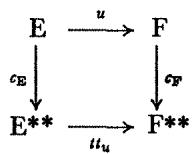
\includegraphics[keepaspectratio]{images/part002_cca49df6.jpg}}

is commutative, as follows immediately from the definitions and formula (15) giving the transpose of a linear mapping.

PROPOSITION 13. If E is a free module (resp. a free module with a finite basis), the canonical mapping \(c_{E}:E \rightarrow E^{**}\) is injective (resp. bijective).

Let \((e_t)_{t \in \mathbb{T}}\) be a basis of \(\mathbf{E}\) and let \((e_t^*)\) be the family of corresponding coordinate forms; by definition, if \(x \in \mathbf{E}\) is such that \(\tilde{x} = 0\) , then \(\langle x, e_t^* \rangle = 0\) for all \(t \in \mathbb{T}\) , in other words all the coordinates of \(x\) are zero, hence \(x = 0\) . Suppose further that \(\mathbf{T}\) is finite; since \(\langle \tilde{e}_t, e_{t'}^* \rangle = \delta_{tt'}\) , \((\tilde{e}_t)\) is the dual basis of \((e_t^*)\) in \(\mathbf{E}^{**}\) and, as \(c_{\mathbf{E}}\) transforms a basis of \(\mathbf{E}\) into a basis of \(\mathbf{E}^{**}\) , \(c_{\mathbf{E}}\) is bijective (§ 1, no. 11, Corollary 3 to Proposition 17). We have moreover proved:

COROLLARY 1. Let E be a free A-module with a finite basis; for every basis \((e_t)\) of E, \((c_{\mathbf{E}}(e_t))\) is the dual basis of the basis \((e_t^*)\) of E* dual to \((e_t)\) .

In this case it is said that \((e_t)\) and \((e_t^*)\) are two dual bases of one another.

COROLLARY 2. If E is a free A-module with a finite basis, every finite basis of \(\mathbf{E}^*\) is the dual basis of a basis of \(\mathbf{E}\) .

It suffices to consider in E** the dual basis of the given basis and canonically to identify E with E**.

COROLLARY 3. Let E, F be two A-modules each with a finite basis, E (resp. F) being canonically identified with its bidual E** (resp. F**). Then, for every linear mapping \(u: \mathbf{E} \to \mathbf{F}\) , \(^{tt}u = u\) .

This follows immediately from the commutativity of diagram (27).

COROLLARY 4. If P is a projective module (resp. a finitely generated projective module) the canonical mapping \(c_{\mathbf{P}}: \mathbf{P} \to \mathbf{P}^{**}\) is injective (resp. bijective).

We shall use the following lemma:

Lemma 1. Let M, N be two supplementary submodules in an A-module E and i: M → E, j: N → E the canonical injections. Then the diagram

\begin{enumerate}
\def\labelenumi{(\arabic{enumi})}
\setcounter{enumi}{27}
\tightlist
\item
\end{enumerate}

\pandocbounded{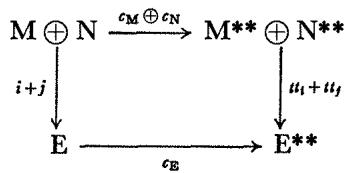
\includegraphics[keepaspectratio]{images/part002_690a791a.jpg}}

is commutative.

By definition, for \(x \in \mathbf{M}\) , \(y \in \mathbf{N}\) , \(z^{*} \in \mathbf{E}^{*}\) ,

\[
\begin{array}{r l} \langle c _ {\mathrm{E}} (i (x) + j (y)), z ^ {*} \rangle & = \langle i (x) + j (y), z ^ {*} \rangle \\ & = \langle i (x), z ^ {*} \rangle + \langle j (y), z ^ {*} \rangle \\ & = \langle x, ^ {t} i (z ^ {*}) \rangle + \langle y, ^ {t} j (z ^ {*}) \rangle \\ & = \langle c _ {\mathrm{M}} (x), ^ {t} i (z ^ {*}) \rangle + \langle c _ {\mathrm{N}} (y), ^ {t} j (z ^ {*}) \rangle \\ & = \langle^ {t t} i (c _ {\mathrm{M}} (x)) + ^ {t t} j (c _ {\mathrm{N}} (y)), z ^ {*} \rangle . \end{array}
\]

This being so, if E is a free module (resp. a free module with a finite basis), \(c_{E}\) is injective (resp. bijective); on the other hand, it follows from no. 6, Proposition 10, that \(^{tt}i \oplus ^{tt}j\) is bijective; the commutativity of diagram (28) then implies that \(c_{M} \oplus c_{N}\) is injective (resp. bijective) and so therefore are \(c_{M}\) and \(c_{N}\) (§ 1, no. 6, Corollary 1 to Proposition 7), whence the corollary, taking account of no. 2, Proposition 4.

\subsection{LINEAR EQUATIONS}

Let E, F be two A-modules. Every equation of the form \(u(x) = y_{0}\) , where \(u: E \to F\) is a given linear mapping, \(y_{0}\) a given element of F and the unknown x is subjected to the condition that it takes its values in E, is called a linear equation; \(y_{0}\) is called the right hand side of the equation; if \(y_{0} = 0\) , the equation is called homogeneous linear.

Every element \(x_{0} \in E\) such that \(u(x_{0}) = y_{0}\) is called a solution of the linear equation \(u(x) = y_{0}\) .†

It is often said, loosely speaking, that a problem is linear if it is equivalent to determining the solutions of a linear equation.

Given a linear equation \(u(x) = y_{0}\) , the equation \(u(x) = 0\) is called the homogeneous linear equation associated with \(u(x) = y_{0}\) .

PROPOSITION 14. If \(x_{0}\) is a solution of the linear equation \(u(x) = y_{0}\) , the set of solutions of this equation is equal to the set of elements \(x_{0} + z\) , where z runs through the set of solutions of the associated homogeneous equation \(u(x) = 0\) .

The relation \(u(x) = y_0\) may be written as \(u(x) = u(x_0)\) , which is equivalent to \(u(x - x_0) = 0\) .

In other words, if the equation \(u(x) = y_{0}\) has at least one solution \(x_{0}\) , the set of its solutions is the set \(x_{0} + u^{-1}(0)\) , obtained by translation from the kernel \(u^{-1}(0)\) of u. Observe that \(u^{-1}(0)\) , being a submodule, is never empty, since it contains 0 (called the zero solution, or trivial solution, of the homogeneous equation \(u(x) = 0\) ).

By virtue of Proposition 14, for a linear equation \(u(x) = y_0\) to have exactly one solution, it is necessary and sufficient that it have at least one solution and that \(u^{-1}(0) = \{0\}\) (in other words, that the associated homogeneous equation have no non-zero solution, or also that \(u\) be injective); in this case, for all \(y \in F\) , the equation \(u(x) = y\) has at most one solution.

PROPOSITION 15. Let \(u\) be a linear mapping of a module \(\mathbf{E}\) into a module \(\mathbf{F}\) . If the equation \(u(x) = y_0\) has at least one solution, \(y_0\) is orthogonal to the kernel of \(^t u\) .

To say that \(u(x) = y_{0}\) admits a solution means that \(y_{0} \in u(\mathbf{E})\) and the proposition follows from no. 5, Corollary to Proposition 8.

Observe that the necessary criterion for the existence of a solution of \(u(x) = y_{0}\) , given by Proposition 15, is sufficient when A is a field (§ 7, no. 6, Proposition 12), but not in general (Exercise 10).

Remarks. (1) Let E be an A-module, \((\mathbf{F}_{i})_{i\in I}\) a family of A-modules and for all \(i\in I\) let \(u_{i}:E\to F_{i}\) be a linear mapping. Every system of linear equations

\[
u _ {i} (x) = y _ {i} \quad (i \in I)\tag{29}
\]

where the \(y_{i} \in \mathbf{F}_{i}\) are given, is equivalent to a single linear equation \(u(x) = y\) , where \(u\) is the mapping \(x \mapsto (u_{i}(x))\) of \(\mathbf{E}\) into \(\mathbf{F} = \prod_{i \in I} \mathbf{F}_{i}\) and \(y = (y_{i})\) . The system (29) is called homogeneous if \(y_{i} = 0\) for all \(i \in I\) .

\begin{enumerate}
\def\labelenumi{(\arabic{enumi})}
\setcounter{enumi}{1}
\tightlist
\item
  Suppose that E admits a basis \((a_{\lambda})_{\lambda \in L}\) ; if we set \(u(a_{\lambda}) = b_{\lambda}\) for all \(\lambda \in L\) , to say that \(x = \sum_{\lambda \in L} \xi_{\lambda} a_{\lambda}\) satisfies the equation \(u(x) = y_0\) is equivalent to saying that the family (of finite support) \((\xi_{\lambda})_{\lambda \in L}\) of elements of A satisfies the relation
\end{enumerate}

\[
\sum_ {\lambda \in L} \xi_ {\lambda} b _ {\lambda} = y _ {0}.\tag{30}
\]

Conversely, looking for families \((\xi_{\lambda})_{\lambda \in L}\) of elements of A of finite support satisfying (30), is equivalent to solving the linear equation \(u(x) = y_0\) , where \(u\) is the unique linear mapping of E into F such that \(u(a_{\lambda}) = b_{\lambda}\) for all \(\lambda \in L\) (§ 1, no. 11, Corollary 3 to Proposition 17).

\begin{enumerate}
\def\labelenumi{(\arabic{enumi})}
\setcounter{enumi}{2}
\tightlist
\item
  A linear equation \(u(x) = y_0\) is called scalar when \(F = A_s\) and therefore \(u\) is a linear form on \(E\) and \(y_0\) a scalar. If \(E\) admits a basis \((a_\lambda)_{\lambda \in L}\) , it follows from Remark (2) that such an equation may also be written as
\end{enumerate}

\[
\sum_ {\lambda \in L} \xi_ {\lambda} \alpha_ {\lambda} = y _ {0} \in A\tag{31}
\]

where the family of scalars \((\alpha_{\lambda})\) is arbitrary and where it is understood that the family \((\xi_{\lambda})\) must have finite support. In general, by the solution (in A) of a system of scalar linear equations

\[
\sum_ {\lambda \in L} \xi_ {\lambda} \alpha_ {\lambda i} = \eta_ {i} \quad (i \in I)\tag{32}
\]

where \(\alpha_{\lambda i} \in A\) and \(\eta_i \in A\) , is understood a family \((\xi_\lambda)_{\lambda \in L}\) of elements of \(A\) of finite support and satisfying (32); the \(\alpha_{\lambda i}\) are called the coefficients of the system of equations and the \(\eta_i\) the right hand sides. The solution of such a system is equivalent to that of the equation \(u(x) = y\) , where \(y = (\eta_i)\) and \(u: A_s^{(L)} \to A_s^I\) is the linear mapping

\[
\left(\xi_ {\lambda}\right) \mapsto \left(\sum_ {\lambda \in L} \xi_ {\lambda} \alpha_ {\lambda i}\right).
\]

\begin{enumerate}
\def\labelenumi{(\arabic{enumi})}
\setcounter{enumi}{3}
\tightlist
\item
  A linear system (32) is also called a system of left scalar linear equations when it is necessary to avoid confusion. A system of equations
\end{enumerate}

\[
\sum_ {\lambda \in L} \alpha_ {\lambda i} \xi_ {\lambda} = \eta_ {i} \quad (i \in I)\tag{33}
\]

is likewise called a system of right scalar linear equations; such a system can immediately be transformed into a system (32) by considering the \(\xi_{\lambda}, \eta_{i}\) and \(\alpha_{\lambda i}\) as belonging to the opposite ring A \(^{0}\) to A.

\section{TENSOR PRODUCTS}

\subsection{TENSOR PRODUCT OF TWO MODULES}

Let \(G_{1}, G_{2}\) be two Z-modules; a mapping u of the set \(G = G_{1} \times G_{2}\) into a Z-module is called biadditive (or Z-bilinear) if \(u(x_{1}, x_{2})\) is ``additive with respect to \(x_{1}\) and with respect to \(x_{2}\) ''; to be precise, this means that, for \(x_{1}, y_{1}\) in \(G_{1}, x_{2}, y_{2}\) in \(G_{2}\) ,

\[
\begin{array}{l} u (x _ {1} + y _ {1}, x _ {2}) = u (x _ {1}, x _ {2}) + u (y _ {1}, x _ {2}) \\ u (x _ {1}, x _ {2} + y _ {2}) = u (x _ {1}, x _ {2}) + u (x _ {1}, y _ {2}). \end{array}
\]

Note that this implies in particular that \(u(0, x_2) = u(x_1, 0) = 0\) for all \(x_1 \in \mathbf{G}_1, x_2 \in \mathbf{G}_2\) .

Let A be a ring, E a right A-module and F a left A-module. We are going to consider the universal mapping problem (Set Theory, IV, § 3, no. 1) where \(\Sigma\) is the species of Z-module structure (the morphisms then being Z-linear mappings, in other words, additive group homomorphisms) and the \(\alpha\) -mappings are the mappings \(f\) of E \(\times\) F into a Z-module G which are Z-bilinear and further satisfy, for all \(x \in \mathbf{E}\) , \(y \in \mathbf{F}\) and \(\lambda \in \mathbf{A}\)

\[
f (x \lambda , y) = f (x, \lambda y).\tag{1}
\]

We show that this problem admits a solution. For this we consider the Z-module \(C = \mathbf{Z}^{(E \times F)}\) of formal linear combinations of the elements of \(E \times F\) with coefficients in Z (§ 1, no. 11), a basis of which can be considered to consist of the ordered pairs \((x, y)\) , where \(x \in E\) and \(y \in F\) . Let D be the sub-Z-module of C generated by the elements of one of the following types:

\[
\left\{ \begin{array}{l} (x _ {1} + x _ {2}, y) - (x _ {1}, y) - (x _ {2}, y) \\ (x, y _ {1} + y _ {2}) - (x, y _ {1}) - (x, y _ {2}) \\ (x \lambda , y) - (x, \lambda y) \end{array} \right.\tag{2}
\]

where \(x, x_{1}, x_{2}\) are in E, \(y, y_{1}, y_{2}\) are in F and \(\lambda\) is in A.

DEFINITION 1. The tensor product of the right A-module E and the left A-module F, denoted by \(\mathbf{E} \otimes_{\mathbf{A}} \mathbf{F}\) or \(\mathbf{E} \otimes_{\mathbf{A}} \mathbf{F}\) (or simply \(\mathbf{E} \otimes \mathbf{F}\) if no confusion is to be feared) is the quotient \(\mathbf{Z}\) -module C/D (the quotient of the \(\mathbf{Z}\) -module C of formal linear combinations of elements of \(\mathbf{E} \times \mathbf{F}\) with coefficients in \(\mathbf{Z}\) , by the submodule \(\mathbf{D}\) generated by the elements of one of the types (2)). For \(x \in \mathbf{E}\) and \(y \in \mathbf{F}\) , the element of \(\mathbf{E} \otimes_{\mathbf{A}} \mathbf{F}\) which is the canonical image of the element \((x, y)\) of \(\mathbf{C} = \mathbf{Z}^{(\mathbf{E} \times \mathbf{F})}\) is denoted by \(x \otimes y\) and called the tensor product of \(x\) and \(y\) .

The mapping \((x,y)\mapsto x\otimes y\) of \(\mathbf{E}\times \mathbf{F}\) into \(\mathbf{E}\otimes_{\mathbf{A}}\mathbf{F}\) is called canonical. It is a Z-bilinear mapping which satisfies conditions (1).

We show that the tensor product \(E \otimes_{A} F\) and the above canonical mapping form a solution of the universal mapping problem posed earlier. To be precise:

PROPOSITION 1. (a) Let \(g\) be a \(\mathbf{Z}\) -linear mapping of \(\mathbf{E} \otimes_{\mathbf{A}} \mathbf{F}\) into a \(\mathbf{Z}\) -module \(\mathbf{G}\) . The mapping \((x, y) \mapsto f(x, y) = g(x \otimes y)\) of \(\mathbf{E} \times \mathbf{F}\) into \(\mathbf{G}\) is \(\mathbf{Z}\) -bilinear and satisfies conditions (1).

\begin{enumerate}
\def\labelenumi{(\alph{enumi})}
\setcounter{enumi}{1}
\tightlist
\item
  Conversely, let \(f\) be a \(\mathbf{Z}\) -bilinear mapping of \(\mathbf{E} \times \mathbf{F}\) into a \(\mathbf{Z}\) -module \(\mathbf{G}\) satisfying conditions (1). Then there exists one and only one \(\mathbf{Z}\) -linear mapping \(g\) of \(\mathbf{E} \otimes_{\mathbf{A}} \mathbf{F}\) into \(\mathbf{G}\) such that \(f(x,y) = g(x \otimes y)\) for \(x \in \mathbf{E}, y \in \mathbf{F}\) .
\end{enumerate}

If \(\phi\) denotes the canonical mapping of \(\mathbf{E} \times \mathbf{F}\) into \(\mathbf{E} \otimes_{\mathbf{A}} \mathbf{F}\) , then \(f = g \circ \phi\) ; whence (a). To show (b), we note that, in the notation of Definition 1, \(f\) extends to a \(\mathbf{Z}\) -linear mapping \(\bar{f}\) of \(\mathbf{C}\) into \(\mathbf{G}\) ( \(\S 1\) , no. 11, Proposition 17). By virtue of relations (1), \(\bar{f}\) is zero for all the elements of \(\mathbf{C}\) of one of the types (2) and hence on \(\mathbf{D}\) . There therefore exists a \(\mathbf{Z}\) -linear mapping \(g\) of \(\mathbf{C} / \mathbf{D} = \mathbf{E} \otimes_{\mathbf{A}} \mathbf{F}\) into \(\mathbf{G}\) such that \(\bar{f} = g \circ \psi\) , where \(\psi: \mathbf{C} \to \mathbf{C} / \mathbf{D}\) is the canonical homomorphism ( \(\S 1\) , no. 8, Remark). The uniqueness of \(g\) is immediate since \(\mathbf{E} \otimes_{\mathbf{A}} \mathbf{F}\) is generated, as a \(\mathbf{Z}\) -module, by the elements of the form \(x \otimes y\) .

Proposition 1 defines a canonical isomorphism of the Z-module of Z-bilinear mappings f of E × F into G, satisfying conditions (1), onto the Z-module Hom \(_{Z}\) (E ⊗A F, G).

When A = Z, conditions (1) are automatically satisfied for every Z-bilinear mapping f and the submodule D of C is already generated by the elements of the first two types in (2).

If now we return to the general case and \(E'\) and \(F'\) denote the underlying Z-modules of E and F respectively, the above remark and Definition 1 show immediately that the Z-module \(E \otimes_{A} F\) can be canonically identified with the quotient of the Z-module \(E' \otimes_{Z} F'\) by the sub-Z-module generated by the elements of the form \((x\lambda) \otimes y - x \otimes (\lambda y)\) , where x runs through E, y runs through F and \(\lambda\) runs through A.

COROLLARY 1. Let H be a Z-module and \(h:E \times F \rightarrow H\) a Z-bilinear mapping satisfying conditions (1) and such that H is generated by \(h(E \times F)\) . Suppose that for every Z-module G and every Z-bilinear mapping f of \(E \times F\) into G satisfying (1)

there exists a Z-linear mapping \(g:H \to G\) such that \(f = g \circ h\) . Then, if \(\phi\) denotes the canonical mapping of \(E \times F\) into \(E \otimes_{A} F\) , there exists one and only one isomorphism \(\theta\) of \(E \otimes_{A} F\) onto H such that \(h = \theta \circ \phi\) .

The hypothesis that \(h(\mathbf{E} \times \mathbf{F})\) generates H implies the uniqueness of g; the corollary is then just the general uniqueness property of a solution of a universal mapping problem (Set Theory, IV, § 3, no. 1).

COROLLARY 2. Let \(\mathbf{E}^0\) (resp. \(\mathbf{F}^0\) ) denote the module \(\mathbf{E}\) (resp. \(\mathbf{F}\) ) considered as a left (resp. right) module over the opposite ring \(\mathbf{A}^0\) ; then there exists one and only one \(\mathbf{Z}\) -module isomorphism \(\sigma: \mathbf{E} \otimes_{\mathbf{A}} \mathbf{F} \to \mathbf{F}^0 \otimes_{\mathbf{A}^0} \mathbf{E}^0\) such that \(\sigma(x \otimes y) = y \otimes x\) for \(x \in \mathbf{E}\) and \(y \in \mathbf{F}\) (``commutativity'' of tensor products).

By definition of the \(A^{0}\) -module structures on \(E^{0}\) and \(F^{0}\) , the mapping \((x,y)\mapsto y\otimes x\) of \(E\times F\) into \(F^{0}\otimes_{A^{0}}E^{0}\) is Z-bilinear and satisfies conditions (1), whence the existence and uniqueness of the Z-linear mapping \(\sigma\) . Similarly a Z-linear mapping \(\tau:F^{0}\otimes_{A^{0}}E^{0}\to E\otimes_{A}F\) is defined such that \(\tau(y\otimes x)=x\otimes y\) and clearly \(\sigma\) and \(\tau\) are inverse isomorphisms.

Remark. The tensor product of non-zero modules may be zero: for example, taking the two Z-modules E = Z/2Z and F = Z/3Z, 2x = 0 and 3y = 0 for all \(x \in E\) and \(y \in F\) ; therefore, in E \(\otimes_{\mathbf{Z}} F\) ,

\[
x \otimes y = 3 (x \otimes y) - 2 (x \otimes y) = x \otimes (3 y) - (2 x) \otimes y = 0
\]

for all \(x\) and \(y\) (cf.~no. 6, Corollary 4 to Proposition 6).

\subsection{TENSOR PRODUCT OF TWO LINEAR MAPPINGS}

Let A be a ring, E, E' two right A-modules, F, F' two left A-modules and \(u: E \rightarrow E'\) and \(v: F \rightarrow F'\) two A-linear mappings. It is easily verified that the mapping

\[
(x, y) \mapsto u (x) \otimes v (y)
\]

of \(\mathbf{E} \times \mathbf{F}\) into \(\mathbf{E}' \otimes_{\mathbf{A}} \mathbf{F}'\) is \(\mathbf{Z}\) -bilinear and satisfies conditions (1) of no. 1. By Proposition 1 of no. 1 there thus exists one and only one \(\mathbf{Z}\) -linear mapping \(w: \mathbf{E} \otimes_{\mathbf{A}} \mathbf{F} \to \mathbf{E}' \otimes_{\mathbf{A}} \mathbf{F}'\) such that

\[
w (x \otimes y) = u (x) \otimes v (y)\tag{3}
\]

for \(x \in \mathbf{E}\) , \(y \in \mathbf{F}\) . This mapping is denoted by \(u \otimes v\) (when no confusion can arise) and is called the tensor product of the linear mappings \(u\) and \(v\) .

It follows immediately from (3) that \((u, v) \mapsto u \otimes v\) is a Z-bilinear mapping called canonical

\[
\operatorname{Hom} _ {\mathbf {A}} (\mathrm{E}, \mathrm{E} ^ {\prime}) \times \operatorname{Hom} _ {\mathbf {A}} (\mathrm{F}, \mathrm{F} ^ {\prime}) \rightarrow \operatorname{Hom} _ {\mathbf {Z}} (\mathrm{E} \otimes_ {\mathbf {A}} \mathrm{F}, \mathrm{E} ^ {\prime} \otimes_ {\mathbf {A}} \mathrm{F} ^ {\prime}).
\]

There corresponds to it by Proposition 1 of no. 1 a \(\mathbf{Z}\) -linear mapping called canonical

\[
\operatorname{Hom} _ {\mathbf {A}} (\mathrm{E}, \mathrm{E} ^ {\prime}) \otimes_ {\mathbf {Z}} \operatorname{Hom} _ {\mathbf {A}} (\mathrm{F}, \mathrm{F} ^ {\prime}) \rightarrow \operatorname{Hom} _ {\mathbf {Z}} (\mathrm{E} \otimes_ {\mathbf {A}} \mathrm{F}, \mathrm{E} ^ {\prime} \otimes_ {\mathbf {A}} \mathrm{F} ^ {\prime})\tag{4}
\]

which associates with every element \(u \otimes v\) of the tensor product the linear mapping \(u \otimes v: \mathbf{E} \otimes_{\mathbf{A}} \mathbf{F} \to \mathbf{E}' \otimes_{\mathbf{A}} \mathbf{F}'\) . Note that the canonical mapping (4) is not necessarily injective nor surjective. The notation \(u \otimes v\) can therefore lead to confusion and it will be necessary for the context to indicate whether it denotes an element of the tensor product or a linear mapping.

Further, let \(\mathbf{E}''\) be a right A-module, \(\mathbf{F}''\) a left A-module and \(u':\mathbf{E}'\to\mathbf{E}''\) , \(v':\mathbf{F}'\to\mathbf{F}''\) A-linear mappings; it follows from (3) that

\[
\left(u ^ {\prime} \circ u\right) \otimes \left(v ^ {\prime} \circ v\right) = \left(u ^ {\prime} \otimes v ^ {\prime}\right) \circ (u \otimes v).\tag{5}
\]
